% MINT paper -- IEEEtran conference, full draft (2026-10-27).
% Story: problem -> gap -> method -> evidence (OPV2V test + unseen town) -> interpretation.
% The previous evaluation-centred draft is kept at archive/main_evaluation_draft.tex (it uses the old
% R1 macro names and no longer compiles against numbers.tex).
%
% Rules for filling this skeleton
%  * Every result number is a macro from numbers.tex or a table from tables/, generated by gen_numbers.py;
%    the forest plot comes from figures/forest.py. Never type a result by hand.
%    Re-run (repository root): python3 paper/gen_numbers.py ; .venv-report/bin/python paper/figures/forest.py
%  * The method is called \mint{} (\mintfull). Never "R1". Its ablation is \mint-noREMOVE.
%    Macro names follow the same rule: ...MINT... (e.g. \VGlobMINTDelta), ...MintNoRem..., \MintClean...
%  * Spell out every abbreviation at first use, in the abstract and again in the body.
%  * Two evaluation sets, always side by side and never pooled: the OPV2V test (primary, confirmatory)
%    and Culver City, an unseen town with the same simulated sensor (secondary, descriptive).
%    Culver City macros are prefixed \Cul (e.g. \CulHeadGlobMINT).
%  * Page budget: abstract to the end of Data and Code Availability at most 9 pages; appendices follow the references.
\documentclass[conference]{IEEEtran}
\IEEEoverridecommandlockouts
\usepackage{cite}
\usepackage{amsmath,amssymb}
\usepackage{graphicx}
\usepackage{booktabs}
\usepackage{array}
\usepackage{placeins}
\usepackage{xcolor}
\usepackage{tikz}
\usetikzlibrary{arrows.meta,positioning,fit,calc}
\usepackage{algorithm}
\usepackage{algpseudocode}
\usepackage{url}
\usepackage[hidelinks]{hyperref}

\newcommand{\TODO}[1]{\textcolor{red}{[TODO: #1]}}
\newcommand{\CITENEEDED}{\textcolor{red}{[CITATION NEEDED]}}
% Method name: change here only.
\newcommand{\mint}{MINT}
\newcommand{\mintfull}{Message INfluence Testing}
\newcommand{\pts}{\,pts}
\newcommand{\dev}{\textsuperscript{dev}}
\newcommand{\Cul}{unseen town (simulated sensor)}
% Table bodies are read with the primitive \@@input: since LaTeX 2020-10 \input is robust, and a
% booktabs rule after an \input'ed tabular body fails with "Misplaced \noalign".
\makeatletter
\newcommand{\tabin}[1]{\@@input #1 }
\makeatother

% generated by paper/gen_numbers.py -- DO NOT EDIT BY HAND
% AP values in AP points (AP x 100); CIs are 95% scenario-bootstrap unless the macro ends in CIblock
\newcommand{\TestScenarios}{15}
\newcommand{\TestFrames}{2{,}066}
\newcommand{\TestFramesRaw}{2066}
\newcommand{\TestNOne}{119}
\newcommand{\TestNTwo}{866}
\newcommand{\TestNThree}{869}
\newcommand{\TestNFourPlus}{212}
\newcommand{\TestNmin}{1}
\newcommand{\TestNmax}{5}
\newcommand{\DevTScenarios}{3}
\newcommand{\DevTFrames}{404}
\newcommand{\DevHScenarios}{4}
\newcommand{\DevHFrames}{371}
\newcommand{\DevTNmin}{2}
\newcommand{\DevTNmax}{4}
\newcommand{\DevHN}{2}
\newcommand{\NumConditions}{12}
\newcommand{\BootB}{2000}
\newcommand{\NumpyOpencoodDiff}{1.9\times 10^{-13}}
\newcommand{\dGlobCleanBRAY}{$-$0.11}
\newcommand{\ciGlobCleanBRAY}{[$-$0.26, $-$0.01]}
\newcommand{\dGlobCleanMINT}{+0.14}
\newcommand{\ciGlobCleanMINT}{[+0.01, +0.31]}
\newcommand{\dGlobCleanMINTNoRem}{$-$0.01}
\newcommand{\ciGlobCleanMINTNoRem}{[$-$0.03, +0.01]}
\newcommand{\dGlobCleanBNORM}{$-$6.13}
\newcommand{\ciGlobCleanBNORM}{[$-$10.03, $-$2.40]}
\newcommand{\dGlobCleanEgo}{$-$21.21}
\newcommand{\ciGlobCleanEgo}{[$-$24.26, $-$17.27]}
\newcommand{\dGlobSpoofFeatBRAY}{+0.51}
\newcommand{\ciGlobSpoofFeatBRAY}{[+0.25, +0.83]}
\newcommand{\dGlobSpoofFeatMINT}{+0.68}
\newcommand{\ciGlobSpoofFeatMINT}{[+0.45, +1.02]}
\newcommand{\dGlobSpoofFeatMINTNoRem}{+0.55}
\newcommand{\ciGlobSpoofFeatMINTNoRem}{[+0.35, +0.82]}
\newcommand{\dGlobSpoofFeatBNORM}{$-$5.95}
\newcommand{\ciGlobSpoofFeatBNORM}{[$-$9.70, $-$2.41]}
\newcommand{\dGlobSpoofFeatEgo}{$-$19.69}
\newcommand{\ciGlobSpoofFeatEgo}{[$-$22.75, $-$15.79]}
\newcommand{\dGlobRemoveFeatBRAY}{$-$0.11}
\newcommand{\ciGlobRemoveFeatBRAY}{[$-$0.27, $-$0.00]}
\newcommand{\dGlobRemoveFeatMINT}{+0.27}
\newcommand{\ciGlobRemoveFeatMINT}{[+0.10, +0.56]}
\newcommand{\dGlobRemoveFeatMINTNoRem}{$-$0.01}
\newcommand{\ciGlobRemoveFeatMINTNoRem}{[$-$0.05, +0.02]}
\newcommand{\dGlobRemoveFeatBNORM}{$-$5.67}
\newcommand{\ciGlobRemoveFeatBNORM}{[$-$9.45, $-$2.13]}
\newcommand{\dGlobRemoveFeatEgo}{$-$20.21}
\newcommand{\ciGlobRemoveFeatEgo}{[$-$23.28, $-$16.15]}
\newcommand{\dGlobShiftFeatBRAY}{+0.17}
\newcommand{\ciGlobShiftFeatBRAY}{[+0.03, +0.36]}
\newcommand{\dGlobShiftFeatMINT}{+0.61}
\newcommand{\ciGlobShiftFeatMINT}{[+0.39, +0.93]}
\newcommand{\dGlobShiftFeatMINTNoRem}{+0.38}
\newcommand{\ciGlobShiftFeatMINTNoRem}{[+0.24, +0.59]}
\newcommand{\dGlobShiftFeatBNORM}{$-$5.61}
\newcommand{\ciGlobShiftFeatBNORM}{[$-$9.33, $-$2.13]}
\newcommand{\dGlobShiftFeatEgo}{$-$19.25}
\newcommand{\ciGlobShiftFeatEgo}{[$-$22.51, $-$15.05]}
\newcommand{\dGlobSpoofPtsBRAY}{+0.02}
\newcommand{\ciGlobSpoofPtsBRAY}{[$-$0.14, +0.13]}
\newcommand{\dGlobSpoofPtsMINT}{+0.25}
\newcommand{\ciGlobSpoofPtsMINT}{[+0.10, +0.44]}
\newcommand{\dGlobSpoofPtsMINTNoRem}{+0.11}
\newcommand{\ciGlobSpoofPtsMINTNoRem}{[+0.06, +0.18]}
\newcommand{\dGlobSpoofPtsBNORM}{$-$6.18}
\newcommand{\ciGlobSpoofPtsBNORM}{[$-$10.06, $-$2.47]}
\newcommand{\dGlobSpoofPtsEgo}{$-$20.94}
\newcommand{\ciGlobSpoofPtsEgo}{[$-$23.95, $-$17.08]}
\newcommand{\dGlobSpoofBlindBRAY}{$-$0.01}
\newcommand{\ciGlobSpoofBlindBRAY}{[$-$0.18, +0.14]}
\newcommand{\dGlobSpoofBlindMINT}{+0.19}
\newcommand{\ciGlobSpoofBlindMINT}{[+0.05, +0.37]}
\newcommand{\dGlobSpoofBlindMINTNoRem}{+0.05}
\newcommand{\ciGlobSpoofBlindMINTNoRem}{[+0.00, +0.11]}
\newcommand{\dGlobSpoofBlindBNORM}{$-$5.81}
\newcommand{\ciGlobSpoofBlindBNORM}{[$-$9.43, $-$2.29]}
\newcommand{\dGlobSpoofBlindEgo}{$-$19.00}
\newcommand{\ciGlobSpoofBlindEgo}{[$-$22.11, $-$15.15]}
\newcommand{\dGlobPgdUntBRAY}{$-$0.02}
\newcommand{\ciGlobPgdUntBRAY}{[$-$0.14, +0.09]}
\newcommand{\dGlobPgdUntMINT}{+0.28}
\newcommand{\ciGlobPgdUntMINT}{[+0.08, +0.58]}
\newcommand{\dGlobPgdUntMINTNoRem}{+0.13}
\newcommand{\ciGlobPgdUntMINTNoRem}{[+0.03, +0.30]}
\newcommand{\dGlobPgdUntBNORM}{$-$8.19}
\newcommand{\ciGlobPgdUntBNORM}{[$-$11.93, $-$4.80]}
\newcommand{\dGlobPgdUntEgo}{$-$17.27}
\newcommand{\ciGlobPgdUntEgo}{[$-$20.15, $-$13.53]}
\newcommand{\dGlobPgdRemBRAY}{$-$0.10}
\newcommand{\ciGlobPgdRemBRAY}{[$-$0.23, $-$0.01]}
\newcommand{\dGlobPgdRemMINT}{+1.22}
\newcommand{\ciGlobPgdRemMINT}{[+0.61, +2.15]}
\newcommand{\dGlobPgdRemMINTNoRem}{$-$0.04}
\newcommand{\ciGlobPgdRemMINTNoRem}{[$-$0.08, $-$0.01]}
\newcommand{\dGlobPgdRemBNORM}{$-$8.89}
\newcommand{\ciGlobPgdRemBNORM}{[$-$13.01, $-$5.08]}
\newcommand{\dGlobPgdRemEgo}{$-$17.97}
\newcommand{\ciGlobPgdRemEgo}{[$-$20.77, $-$14.14]}
\newcommand{\dGlobPgdUntStBRAY}{$-$0.06}
\newcommand{\ciGlobPgdUntStBRAY}{[$-$0.21, +0.05]}
\newcommand{\dGlobPgdUntStMINT}{+0.20}
\newcommand{\ciGlobPgdUntStMINT}{[+0.03, +0.46]}
\newcommand{\dGlobPgdUntStMINTNoRem}{+0.06}
\newcommand{\ciGlobPgdUntStMINTNoRem}{[$-$0.03, +0.17]}
\newcommand{\dGlobPgdUntStBNORM}{$-$2.83}
\newcommand{\ciGlobPgdUntStBNORM}{[$-$4.94, $-$0.80]}
\newcommand{\dGlobPgdUntStEgo}{$-$18.45}
\newcommand{\ciGlobPgdUntStEgo}{[$-$21.49, $-$14.47]}
\newcommand{\dGlobPgdRemStBRAY}{$-$0.10}
\newcommand{\ciGlobPgdRemStBRAY}{[$-$0.24, $-$0.01]}
\newcommand{\dGlobPgdRemStMINT}{+1.13}
\newcommand{\ciGlobPgdRemStMINT}{[+0.55, +1.99]}
\newcommand{\dGlobPgdRemStMINTNoRem}{$-$0.04}
\newcommand{\ciGlobPgdRemStMINTNoRem}{[$-$0.09, $-$0.01]}
\newcommand{\dGlobPgdRemStBNORM}{$-$2.61}
\newcommand{\ciGlobPgdRemStBNORM}{[$-$4.14, $-$1.06]}
\newcommand{\dGlobPgdRemStEgo}{$-$18.15}
\newcommand{\ciGlobPgdRemStEgo}{[$-$20.98, $-$14.29]}
\newcommand{\dGlobPgdUntStStrongBRAY}{+0.12}
\newcommand{\ciGlobPgdUntStStrongBRAY}{[$-$0.02, +0.30]}
\newcommand{\dGlobPgdUntStStrongMINT}{+0.40}
\newcommand{\ciGlobPgdUntStStrongMINT}{[+0.14, +0.80]}
\newcommand{\dGlobPgdUntStStrongMINTNoRem}{+0.33}
\newcommand{\ciGlobPgdUntStStrongMINTNoRem}{[+0.12, +0.66]}
\newcommand{\dGlobPgdUntStStrongBNORM}{$-$4.32}
\newcommand{\ciGlobPgdUntStStrongBNORM}{[$-$7.28, $-$1.37]}
\newcommand{\dGlobPgdUntStStrongEgo}{$-$12.36}
\newcommand{\ciGlobPgdUntStStrongEgo}{[$-$16.32, $-$7.39]}
\newcommand{\dGlobPgdRemStStrongBRAY}{$-$0.01}
\newcommand{\ciGlobPgdRemStStrongBRAY}{[$-$0.05, +0.02]}
\newcommand{\dGlobPgdRemStStrongMINT}{+22.50}
\newcommand{\ciGlobPgdRemStStrongMINT}{[+18.41, +27.48]}
\newcommand{\dGlobPgdRemStStrongMINTNoRem}{+0.07}
\newcommand{\ciGlobPgdRemStStrongMINTNoRem}{[+0.01, +0.14]}
\newcommand{\dGlobPgdRemStStrongBNORM}{$-$3.06}
\newcommand{\ciGlobPgdRemStStrongBNORM}{[$-$5.36, $-$1.03]}
\newcommand{\dGlobPgdRemStStrongEgo}{+19.19}
\newcommand{\ciGlobPgdRemStStrongEgo}{[+14.29, +25.04]}
\newcommand{\dFrameCleanBRAY}{+0.04}
\newcommand{\ciFrameCleanBRAY}{[$-$0.15, +0.24]}
\newcommand{\dFrameCleanMINT}{$-$0.51}
\newcommand{\ciFrameCleanMINT}{[$-$1.44, $-$0.15]}
\newcommand{\dFrameCleanMINTNoRem}{+0.03}
\newcommand{\ciFrameCleanMINTNoRem}{[+0.01, +0.08]}
\newcommand{\dFrameCleanBNORM}{$-$7.76}
\newcommand{\ciFrameCleanBNORM}{[$-$12.97, $-$3.07]}
\newcommand{\dFrameCleanEgo}{$-$26.52}
\newcommand{\ciFrameCleanEgo}{[$-$31.42, $-$21.36]}
\newcommand{\dFrameSpoofFeatBRAY}{+1.47}
\newcommand{\ciFrameSpoofFeatBRAY}{[+0.96, +2.41]}
\newcommand{\dFrameSpoofFeatMINT}{+0.68}
\newcommand{\ciFrameSpoofFeatMINT}{[+0.21, +1.12]}
\newcommand{\dFrameSpoofFeatMINTNoRem}{+1.20}
\newcommand{\ciFrameSpoofFeatMINTNoRem}{[+0.83, +1.94]}
\newcommand{\dFrameSpoofFeatBNORM}{$-$6.93}
\newcommand{\ciFrameSpoofFeatBNORM}{[$-$11.57, $-$2.54]}
\newcommand{\dFrameSpoofFeatEgo}{$-$22.95}
\newcommand{\ciFrameSpoofFeatEgo}{[$-$28.09, $-$17.45]}
\newcommand{\dFrameRemoveFeatBRAY}{+0.05}
\newcommand{\ciFrameRemoveFeatBRAY}{[$-$0.12, +0.24]}
\newcommand{\dFrameRemoveFeatMINT}{$-$0.38}
\newcommand{\ciFrameRemoveFeatMINT}{[$-$1.31, +0.05]}
\newcommand{\dFrameRemoveFeatMINTNoRem}{+0.04}
\newcommand{\ciFrameRemoveFeatMINTNoRem}{[+0.00, +0.11]}
\newcommand{\dFrameRemoveFeatBNORM}{$-$7.16}
\newcommand{\ciFrameRemoveFeatBNORM}{[$-$12.02, $-$2.69]}
\newcommand{\dFrameRemoveFeatEgo}{$-$25.36}
\newcommand{\ciFrameRemoveFeatEgo}{[$-$30.51, $-$19.82]}
\newcommand{\dFrameShiftFeatBRAY}{+1.00}
\newcommand{\ciFrameShiftFeatBRAY}{[+0.55, +1.78]}
\newcommand{\dFrameShiftFeatMINT}{+0.55}
\newcommand{\ciFrameShiftFeatMINT}{[$-$0.22, +1.16]}
\newcommand{\dFrameShiftFeatMINTNoRem}{+0.99}
\newcommand{\ciFrameShiftFeatMINTNoRem}{[+0.53, +1.67]}
\newcommand{\dFrameShiftFeatBNORM}{$-$6.73}
\newcommand{\ciFrameShiftFeatBNORM}{[$-$11.19, $-$2.64]}
\newcommand{\dFrameShiftFeatEgo}{$-$23.11}
\newcommand{\ciFrameShiftFeatEgo}{[$-$28.87, $-$17.25]}
\newcommand{\dFrameSpoofPtsBRAY}{+0.51}
\newcommand{\ciFrameSpoofPtsBRAY}{[+0.26, +0.98]}
\newcommand{\dFrameSpoofPtsMINT}{$-$0.09}
\newcommand{\ciFrameSpoofPtsMINT}{[$-$0.77, +0.20]}
\newcommand{\dFrameSpoofPtsMINTNoRem}{+0.43}
\newcommand{\ciFrameSpoofPtsMINTNoRem}{[+0.31, +0.73]}
\newcommand{\dFrameSpoofPtsBNORM}{$-$7.69}
\newcommand{\ciFrameSpoofPtsBNORM}{[$-$12.62, $-$3.00]}
\newcommand{\dFrameSpoofPtsEgo}{$-$25.40}
\newcommand{\ciFrameSpoofPtsEgo}{[$-$30.41, $-$20.13]}
\newcommand{\dFrameSpoofBlindBRAY}{+0.14}
\newcommand{\ciFrameSpoofBlindBRAY}{[$-$0.05, +0.41]}
\newcommand{\dFrameSpoofBlindMINT}{$-$0.34}
\newcommand{\ciFrameSpoofBlindMINT}{[$-$1.04, $-$0.02]}
\newcommand{\dFrameSpoofBlindMINTNoRem}{+0.11}
\newcommand{\ciFrameSpoofBlindMINTNoRem}{[+0.05, +0.24]}
\newcommand{\dFrameSpoofBlindBNORM}{$-$6.70}
\newcommand{\ciFrameSpoofBlindBNORM}{[$-$11.23, $-$2.38]}
\newcommand{\dFrameSpoofBlindEgo}{$-$22.13}
\newcommand{\ciFrameSpoofBlindEgo}{[$-$27.04, $-$16.81]}
\newcommand{\dFramePgdUntBRAY}{+0.83}
\newcommand{\ciFramePgdUntBRAY}{[+0.40, +1.57]}
\newcommand{\dFramePgdUntMINT}{+0.24}
\newcommand{\ciFramePgdUntMINT}{[$-$0.51, +0.77]}
\newcommand{\dFramePgdUntMINTNoRem}{+0.76}
\newcommand{\ciFramePgdUntMINTNoRem}{[+0.44, +1.38]}
\newcommand{\dFramePgdUntBNORM}{$-$3.64}
\newcommand{\ciFramePgdUntBNORM}{[$-$7.72, $-$0.92]}
\newcommand{\dFramePgdUntEgo}{$-$15.50}
\newcommand{\ciFramePgdUntEgo}{[$-$22.71, $-$8.70]}
\newcommand{\dFramePgdRemBRAY}{$-$0.02}
\newcommand{\ciFramePgdRemBRAY}{[$-$0.19, +0.10]}
\newcommand{\dFramePgdRemMINT}{$-$0.07}
\newcommand{\ciFramePgdRemMINT}{[$-$1.34, +0.84]}
\newcommand{\dFramePgdRemMINTNoRem}{$-$0.03}
\newcommand{\ciFramePgdRemMINTNoRem}{[$-$0.06, +0.01]}
\newcommand{\dFramePgdRemBNORM}{$-$13.40}
\newcommand{\ciFramePgdRemBNORM}{[$-$19.41, $-$8.43]}
\newcommand{\dFramePgdRemEgo}{$-$25.26}
\newcommand{\ciFramePgdRemEgo}{[$-$30.23, $-$20.36]}
\newcommand{\dFramePgdUntStBRAY}{+0.58}
\newcommand{\ciFramePgdUntStBRAY}{[+0.16, +1.34]}
\newcommand{\dFramePgdUntStMINT}{+0.03}
\newcommand{\ciFramePgdUntStMINT}{[$-$0.65, +0.53]}
\newcommand{\dFramePgdUntStMINTNoRem}{+0.53}
\newcommand{\ciFramePgdUntStMINTNoRem}{[+0.24, +1.07]}
\newcommand{\dFramePgdUntStBNORM}{$-$4.00}
\newcommand{\ciFramePgdUntStBNORM}{[$-$7.69, $-$1.01]}
\newcommand{\dFramePgdUntStEgo}{$-$19.00}
\newcommand{\ciFramePgdUntStEgo}{[$-$25.85, $-$11.66]}
\newcommand{\dFramePgdRemStBRAY}{$-$0.02}
\newcommand{\ciFramePgdRemStBRAY}{[$-$0.20, +0.12]}
\newcommand{\dFramePgdRemStMINT}{$-$0.14}
\newcommand{\ciFramePgdRemStMINT}{[$-$1.40, +0.73]}
\newcommand{\dFramePgdRemStMINTNoRem}{$-$0.02}
\newcommand{\ciFramePgdRemStMINTNoRem}{[$-$0.06, +0.01]}
\newcommand{\dFramePgdRemStBNORM}{$-$3.51}
\newcommand{\ciFramePgdRemStBNORM}{[$-$5.76, $-$1.40]}
\newcommand{\dFramePgdRemStEgo}{$-$25.38}
\newcommand{\ciFramePgdRemStEgo}{[$-$30.51, $-$20.36]}
\newcommand{\dFramePgdUntStStrongBRAY}{+2.09}
\newcommand{\ciFramePgdUntStStrongBRAY}{[+1.00, +3.70]}
\newcommand{\dFramePgdUntStStrongMINT}{+1.33}
\newcommand{\ciFramePgdUntStStrongMINT}{[+0.19, +2.44]}
\newcommand{\dFramePgdUntStStrongMINTNoRem}{+1.93}
\newcommand{\ciFramePgdUntStStrongMINTNoRem}{[+1.01, +3.27]}
\newcommand{\dFramePgdUntStStrongBNORM}{$-$5.87}
\newcommand{\ciFramePgdUntStStrongBNORM}{[$-$10.77, $-$1.58]}
\newcommand{\dFramePgdUntStStrongEgo}{$-$6.42}
\newcommand{\ciFramePgdUntStStrongEgo}{[$-$17.85, +3.34]}
\newcommand{\dFramePgdRemStStrongBRAY}{+0.06}
\newcommand{\ciFramePgdRemStStrongBRAY}{[$-$0.01, +0.14]}
\newcommand{\dFramePgdRemStStrongMINT}{+20.94}
\newcommand{\ciFramePgdRemStStrongMINT}{[+16.96, +25.78]}
\newcommand{\dFramePgdRemStStrongMINTNoRem}{+0.10}
\newcommand{\ciFramePgdRemStStrongMINTNoRem}{[+0.04, +0.19]}
\newcommand{\dFramePgdRemStStrongBNORM}{$-$3.62}
\newcommand{\ciFramePgdRemStStrongBNORM}{[$-$6.63, $-$1.13]}
\newcommand{\dFramePgdRemStStrongEgo}{+9.99}
\newcommand{\ciFramePgdRemStStrongEgo}{[+3.88, +16.79]}
\newcommand{\RestoredGlobPgdRemStStrongMINT}{22.50}
\newcommand{\HeadGlobBRAY}{+0.15}
\newcommand{\HeadGlobBRAYCI}{[$-$0.01, +0.30]}
\newcommand{\HeadGlobBRAYCIblock}{[+0.06, +0.22]}
\newcommand{\HeadGlobMINT}{+0.45}
\newcommand{\HeadGlobMINTCI}{[+0.29, +0.70]}
\newcommand{\HeadGlobMINTCIblock}{[+0.37, +0.54]}
\newcommand{\HeadGlobMINTNoRem}{+0.26}
\newcommand{\HeadGlobMINTNoRemCI}{[+0.18, +0.36]}
\newcommand{\HeadGlobMINTNoRemCIblock}{[+0.21, +0.30]}
\newcommand{\HeadGlobBNORM}{$-$5.85}
\newcommand{\HeadGlobBNORMCI}{[$-$9.65, $-$2.30]}
\newcommand{\HeadGlobBNORMCIblock}{[$-$7.04, $-$4.63]}
\newcommand{\HeadFrameBRAY}{+0.76}
\newcommand{\HeadFrameBRAYCI}{[+0.49, +1.27]}
\newcommand{\HeadFrameBRAYCIblock}{[+0.63, +0.90]}
\newcommand{\HeadFrameMINT}{+0.19}
\newcommand{\HeadFrameMINTCI}{[$-$0.45, +0.52]}
\newcommand{\HeadFrameMINTCIblock}{[$-$0.00, +0.35]}
\newcommand{\HeadFrameMINTNoRem}{+0.66}
\newcommand{\HeadFrameMINTNoRemCI}{[+0.48, +1.03]}
\newcommand{\HeadFrameMINTNoRemCIblock}{[+0.57, +0.77]}
\newcommand{\HeadFrameBNORM}{$-$7.13}
\newcommand{\HeadFrameBNORMCI}{[$-$11.82, $-$2.73]}
\newcommand{\HeadFrameBNORMCIblock}{[$-$8.61, $-$5.63]}
\newcommand{\HeadGlobEgo}{$-$20.02}
\newcommand{\HeadGlobEgoCI}{[$-$23.10, $-$16.04]}
\newcommand{\HeadGlobEgoCIblock}{[$-$21.08, $-$18.94]}
\newcommand{\HeadFrameEgo}{$-$24.20}
\newcommand{\HeadFrameEgoCI}{[$-$29.44, $-$18.65]}
\newcommand{\HeadFrameEgoCIblock}{[$-$25.62, $-$22.75]}
\newcommand{\VGlobBRAYDelta}{+0.15}
\newcommand{\VGlobBRAYCI}{[$-$0.01, +0.30]}
\newcommand{\VGlobBRAYCIblock}{[+0.06, +0.22]}
\newcommand{\VGlobBRAYP}{0.0335}
\newcommand{\VGlobBRAYHolmRank}{2}
\newcommand{\VGlobBRAYHolmThr}{0.050}
\newcommand{\VGlobBRAYReject}{yes}
\newcommand{\VGlobBRAYK}{66}
\newcommand{\VGlobMINTDelta}{+0.45}
\newcommand{\VGlobMINTCI}{[+0.29, +0.70]}
\newcommand{\VGlobMINTCIblock}{[+0.37, +0.54]}
\newcommand{\VGlobMINTP}{0.0005}
\newcommand{\VGlobMINTHolmRank}{1}
\newcommand{\VGlobMINTHolmThr}{0.025}
\newcommand{\VGlobMINTReject}{yes}
\newcommand{\VGlobMINTK}{0}
\newcommand{\VGlobBRAYCleanLoss}{0.13\%}
\newcommand{\VGlobBRAYCleanCI}{[+0.01, +0.30]\%}
\newcommand{\VGlobCleanOK}{yes}
\newcommand{\VGlobPass}{passes}
\newcommand{\VGlobRmB}{+0.31}
\newcommand{\VGlobRmBCI}{[+0.12, +0.55]}
\newcommand{\VGlobRmBCIblock}{[+0.22, +0.40]}
\newcommand{\VGlobRmBStatement}{the counterfactual improves over the box-level filter}
\newcommand{\VFrameBRAYDelta}{+0.76}
\newcommand{\VFrameBRAYCI}{[+0.49, +1.27]}
\newcommand{\VFrameBRAYCIblock}{[+0.63, +0.90]}
\newcommand{\VFrameBRAYP}{0.0005}
\newcommand{\VFrameBRAYHolmRank}{1}
\newcommand{\VFrameBRAYHolmThr}{0.025}
\newcommand{\VFrameBRAYReject}{yes}
\newcommand{\VFrameBRAYK}{0}
\newcommand{\VFrameMINTDelta}{+0.19}
\newcommand{\VFrameMINTCI}{[$-$0.45, +0.52]}
\newcommand{\VFrameMINTCIblock}{[$-$0.00, +0.35]}
\newcommand{\VFrameMINTP}{0.2259}
\newcommand{\VFrameMINTHolmRank}{2}
\newcommand{\VFrameMINTHolmThr}{0.050}
\newcommand{\VFrameMINTReject}{no}
\newcommand{\VFrameMINTK}{451}
\newcommand{\VFrameBRAYCleanLoss}{$-$0.05\%}
\newcommand{\VFrameBRAYCleanCI}{[$-$0.30, +0.18]\%}
\newcommand{\VFrameCleanOK}{yes}
\newcommand{\VFramePass}{passes}
\newcommand{\VFrameRmB}{$-$0.57}
\newcommand{\VFrameRmBCI}{[$-$1.64, $-$0.11]}
\newcommand{\VFrameRmBCIblock}{[$-$0.75, $-$0.43]}
\newcommand{\VFrameRmBStatement}{the counterfactual performs worse than the box-level filter}
\newcommand{\BothPass}{yes}
\newcommand{\CleanGlobBRAY}{0.13\%}
\newcommand{\CleanGlobBRAYCI}{[+0.01, +0.30]\%}
\newcommand{\CleanGlobMINT}{$-$0.16\%}
\newcommand{\CleanGlobMINTCI}{[$-$0.35, $-$0.01]\%}
\newcommand{\CleanGlobMINTNoRem}{0.01\%}
\newcommand{\CleanGlobMINTNoRemCI}{[$-$0.01, +0.03]\%}
\newcommand{\CleanGlobBNORM}{6.92\%}
\newcommand{\CleanGlobBNORMCI}{[+2.72, +11.33]\%}
\newcommand{\CleanFrameBRAY}{$-$0.05\%}
\newcommand{\CleanFrameBRAYCI}{[$-$0.30, +0.18]\%}
\newcommand{\CleanFrameMINT}{0.62\%}
\newcommand{\CleanFrameMINTCI}{[+0.18, +1.75]\%}
\newcommand{\CleanFrameMINTNoRem}{$-$0.03\%}
\newcommand{\CleanFrameMINTNoRemCI}{[$-$0.10, $-$0.01]\%}
\newcommand{\CleanFrameBNORM}{9.45\%}
\newcommand{\CleanFrameBNORMCI}{[+3.66, +15.70]\%}
\newcommand{\CleanGlobEgo}{23.93\%}
\newcommand{\CleanGlobEgoCI}{[+19.84, +27.10]\%}
\newcommand{\CleanFrameEgo}{32.27\%}
\newcommand{\CleanFrameEgoCI}{[+26.89, +37.04]\%}
\newcommand{\MintCleanUnits}{8160}
\newcommand{\MintCleanKnown}{53\%}
\newcommand{\MintCleanGated}{718}
\newcommand{\MintCleanGatedHarmful}{190}
\newcommand{\MintCleanFalseSwitch}{521}
\newcommand{\MintCleanFalseSwitchRemove}{512}
\newcommand{\MintCleanGatedRemove}{657}
\newcommand{\MintCleanPrecision}{0.27}
\newcommand{\MintNoRemCleanGated}{62}
\newcommand{\MintNoRemCleanFalseSwitch}{10}
\newcommand{\MintNoRemCleanPrecision}{0.73}
\newcommand{\BrayCleanBoxes}{31{,}106}
\newcommand{\BrayCleanDrop}{148}
\newcommand{\BrayCleanDropGT}{43}
\newcommand{\BrayCleanKnown}{84\%}
\newcommand{\BnormFalseFlag}{17.4\%}
\newcommand{\BnormFalseFlagN}{339}
\newcommand{\BnormFramesWithSender}{1947}
\newcommand{\BnormFalseFlagH}{1.6\%}
\newcommand{\BnormTauOne}{1.020}
\newcommand{\BnormTauThree}{1.195}
\newcommand{\RmBGlobMeanThree}{+0.28}
\newcommand{\RmBGlobMeanThreeCI}{[+0.10, +0.50]}
\newcommand{\RmBGlobClean}{+0.25}
\newcommand{\RmBGlobCleanCI}{[+0.07, +0.47]}
\newcommand{\RmBGlobSpoofFeat}{+0.18}
\newcommand{\RmBGlobSpoofFeatCI}{[+0.01, +0.38]}
\newcommand{\RmBGlobRemoveFeat}{+0.38}
\newcommand{\RmBGlobRemoveFeatCI}{[+0.16, +0.69]}
\newcommand{\RmBGlobShiftFeat}{+0.44}
\newcommand{\RmBGlobShiftFeatCI}{[+0.21, +0.70]}
\newcommand{\RmBGlobSpoofPts}{+0.23}
\newcommand{\RmBGlobSpoofPtsCI}{[+0.06, +0.44]}
\newcommand{\RmBGlobSpoofBlind}{+0.20}
\newcommand{\RmBGlobSpoofBlindCI}{[+0.04, +0.41]}
\newcommand{\RmBFrameMeanThree}{$-$0.61}
\newcommand{\RmBFrameMeanThreeCI}{[$-$1.69, $-$0.16]}
\newcommand{\RmBFrameClean}{$-$0.55}
\newcommand{\RmBFrameCleanCI}{[$-$1.58, $-$0.11]}
\newcommand{\RmBFrameSpoofFeat}{$-$0.79}
\newcommand{\RmBFrameSpoofFeatCI}{[$-$1.85, $-$0.34]}
\newcommand{\RmBFrameRemoveFeat}{$-$0.44}
\newcommand{\RmBFrameRemoveFeatCI}{[$-$1.47, +0.02]}
\newcommand{\RmBFrameShiftFeat}{$-$0.45}
\newcommand{\RmBFrameShiftFeatCI}{[$-$1.54, +0.03]}
\newcommand{\RmBFrameSpoofPts}{$-$0.61}
\newcommand{\RmBFrameSpoofPtsCI}{[$-$1.67, $-$0.16]}
\newcommand{\RmBFrameSpoofBlind}{$-$0.48}
\newcommand{\RmBFrameSpoofBlindCI}{[$-$1.38, $-$0.07]}
\newcommand{\RmBGlobPgdUnt}{+0.30}
\newcommand{\RmBGlobPgdUntCI}{[+0.09, +0.58]}
\newcommand{\RmBGlobPgdRem}{+1.31}
\newcommand{\RmBGlobPgdRemCI}{[+0.68, +2.24]}
\newcommand{\RmBGlobPgdUntSt}{+0.26}
\newcommand{\RmBGlobPgdUntStCI}{[+0.07, +0.51]}
\newcommand{\RmBGlobPgdRemSt}{+1.24}
\newcommand{\RmBGlobPgdRemStCI}{[+0.64, +2.10]}
\newcommand{\RmBGlobPgdUntStStrong}{+0.27}
\newcommand{\RmBGlobPgdUntStStrongCI}{[+0.03, +0.60]}
\newcommand{\RmBGlobPgdRemStStrong}{+22.51}
\newcommand{\RmBGlobPgdRemStStrongCI}{[+18.40, +27.52]}
\newcommand{\RmBFramePgdUnt}{$-$0.59}
\newcommand{\RmBFramePgdUntCI}{[$-$1.63, $-$0.13]}
\newcommand{\RmBFramePgdRem}{$-$0.05}
\newcommand{\RmBFramePgdRemCI}{[$-$1.38, +0.93]}
\newcommand{\RmBFramePgdUntSt}{$-$0.55}
\newcommand{\RmBFramePgdUntStCI}{[$-$1.54, $-$0.10]}
\newcommand{\RmBFramePgdRemSt}{$-$0.12}
\newcommand{\RmBFramePgdRemStCI}{[$-$1.41, +0.80]}
\newcommand{\RmBFramePgdUntStStrong}{$-$0.76}
\newcommand{\RmBFramePgdUntStStrongCI}{[$-$1.83, $-$0.25]}
\newcommand{\RmBFramePgdRemStStrong}{+20.88}
\newcommand{\RmBFramePgdRemStStrongCI}{[+16.84, +25.73]}
\newcommand{\LossGlobSpoofFeat}{1.52}
\newcommand{\LossGlobRemoveFeat}{1.01}
\newcommand{\LossGlobShiftFeat}{1.97}
\newcommand{\LossGlobSpoofPts}{0.27}
\newcommand{\LossGlobSpoofBlind}{2.21}
\newcommand{\LossGlobPgdUnt}{3.95}
\newcommand{\LossGlobPgdRem}{3.25}
\newcommand{\LossGlobPgdUntSt}{2.77}
\newcommand{\LossGlobPgdRemSt}{3.06}
\newcommand{\LossGlobPgdUntStStrong}{8.86}
\newcommand{\LossGlobPgdRemStStrong}{40.41}
\newcommand{\LossFrameSpoofFeat}{3.57}
\newcommand{\LossFrameRemoveFeat}{1.16}
\newcommand{\LossFrameShiftFeat}{3.40}
\newcommand{\LossFrameSpoofPts}{1.11}
\newcommand{\LossFrameSpoofBlind}{4.39}
\newcommand{\LossFramePgdUnt}{11.02}
\newcommand{\LossFramePgdRem}{1.26}
\newcommand{\LossFramePgdUntSt}{7.52}
\newcommand{\LossFramePgdRemSt}{1.14}
\newcommand{\LossFramePgdUntStStrong}{20.10}
\newcommand{\LossFramePgdRemStStrong}{36.51}
\newcommand{\AppliedSpoofFeat}{1921}
\newcommand{\RealizedSpoofFeat}{1136}
\newcommand{\WithSenderSpoofFeat}{1947}
\newcommand{\AppliedRemoveFeat}{1921}
\newcommand{\RealizedRemoveFeat}{176}
\newcommand{\WithSenderRemoveFeat}{1947}
\newcommand{\AppliedShiftFeat}{1914}
\newcommand{\RealizedShiftFeat}{206}
\newcommand{\WithSenderShiftFeat}{1947}
\newcommand{\AppliedSpoofPts}{1895}
\newcommand{\RealizedSpoofPts}{563}
\newcommand{\WithSenderSpoofPts}{1947}
\newcommand{\AppliedSpoofBlind}{1925}
\newcommand{\RealizedSpoofBlind}{1412}
\newcommand{\WithSenderSpoofBlind}{1947}
\newcommand{\AppliedPgdUnt}{1947}
\newcommand{\RealizedPgdUnt}{1541}
\newcommand{\WithSenderPgdUnt}{1947}
\newcommand{\InfeasiblePgdUnt}{0}
\newcommand{\AppliedPgdRem}{1947}
\newcommand{\RealizedPgdRem}{1233}
\newcommand{\WithSenderPgdRem}{1947}
\newcommand{\InfeasiblePgdRem}{0}
\newcommand{\AppliedPgdUntSt}{1937}
\newcommand{\RealizedPgdUntSt}{1402}
\newcommand{\WithSenderPgdUntSt}{1947}
\newcommand{\InfeasiblePgdUntSt}{10}
\newcommand{\AppliedPgdRemSt}{1903}
\newcommand{\RealizedPgdRemSt}{1193}
\newcommand{\WithSenderPgdRemSt}{1947}
\newcommand{\InfeasiblePgdRemSt}{44}
\newcommand{\AppliedPgdUntStStrong}{1944}
\newcommand{\RealizedPgdUntStStrong}{1709}
\newcommand{\WithSenderPgdUntStStrong}{1947}
\newcommand{\InfeasiblePgdUntStStrong}{3}
\newcommand{\AppliedPgdRemStStrong}{1944}
\newcommand{\RealizedPgdRemStStrong}{1944}
\newcommand{\WithSenderPgdRemStStrong}{1947}
\newcommand{\InfeasiblePgdRemStStrong}{3}
\newcommand{\BlindRealizedLowRay}{1381}
\newcommand{\BlindRealizedKnownHit}{0}
\newcommand{\RecGlobPgdUntBRAY}{$-$0.00}
\newcommand{\RecGlobPgdUntMINT}{0.07}
\newcommand{\RecGlobPgdUntMINTNoRem}{0.03}
\newcommand{\RecGlobPgdUntBNORM}{$-$2.07}
\newcommand{\RecGlobPgdRemBRAY}{$-$0.03}
\newcommand{\RecGlobPgdRemMINT}{0.37}
\newcommand{\RecGlobPgdRemMINTNoRem}{$-$0.01}
\newcommand{\RecGlobPgdRemBNORM}{$-$2.74}
\newcommand{\RecGlobPgdUntStBRAY}{$-$0.02}
\newcommand{\RecGlobPgdUntStMINT}{0.07}
\newcommand{\RecGlobPgdUntStMINTNoRem}{0.02}
\newcommand{\RecGlobPgdUntStBNORM}{$-$1.02}
\newcommand{\RecGlobPgdRemStBRAY}{$-$0.03}
\newcommand{\RecGlobPgdRemStMINT}{0.37}
\newcommand{\RecGlobPgdRemStMINTNoRem}{$-$0.01}
\newcommand{\RecGlobPgdRemStBNORM}{$-$0.85}
\newcommand{\RecGlobPgdUntStStrongBRAY}{0.01}
\newcommand{\RecGlobPgdUntStStrongMINT}{0.04}
\newcommand{\RecGlobPgdUntStStrongMINTNoRem}{0.04}
\newcommand{\RecGlobPgdUntStStrongBNORM}{$-$0.49}
\newcommand{\RecGlobPgdRemStStrongBRAY}{$-$0.00}
\newcommand{\RecGlobPgdRemStStrongMINT}{0.56}
\newcommand{\RecGlobPgdRemStStrongMINTNoRem}{0.00}
\newcommand{\RecGlobPgdRemStStrongBNORM}{$-$0.08}
\newcommand{\RecFramePgdUntBRAY}{0.08}
\newcommand{\RecFramePgdUntMINT}{0.02}
\newcommand{\RecFramePgdUntMINTNoRem}{0.07}
\newcommand{\RecFramePgdUntBNORM}{$-$0.33}
\newcommand{\RecFramePgdRemBRAY}{$-$0.02}
\newcommand{\RecFramePgdRemMINT}{$-$0.05}
\newcommand{\RecFramePgdRemMINTNoRem}{$-$0.02}
\newcommand{\RecFramePgdRemBNORM}{$-$10.66}
\newcommand{\RecFramePgdUntStBRAY}{0.08}
\newcommand{\RecFramePgdUntStMINT}{0.00}
\newcommand{\RecFramePgdUntStMINTNoRem}{0.07}
\newcommand{\RecFramePgdUntStBNORM}{$-$0.53}
\newcommand{\RecFramePgdRemStBRAY}{$-$0.02}
\newcommand{\RecFramePgdRemStMINT}{$-$0.13}
\newcommand{\RecFramePgdRemStMINTNoRem}{$-$0.02}
\newcommand{\RecFramePgdRemStBNORM}{$-$3.09}
\newcommand{\RecFramePgdUntStStrongBRAY}{0.10}
\newcommand{\RecFramePgdUntStStrongMINT}{0.07}
\newcommand{\RecFramePgdUntStStrongMINTNoRem}{0.10}
\newcommand{\RecFramePgdUntStStrongBNORM}{$-$0.29}
\newcommand{\RecFramePgdRemStStrongBRAY}{0.00}
\newcommand{\RecFramePgdRemStStrongMINT}{0.57}
\newcommand{\RecFramePgdRemStStrongMINTNoRem}{0.00}
\newcommand{\RecFramePgdRemStStrongBNORM}{$-$0.10}
\newcommand{\RecGlobPgdRemStStrongMINTexp}{0.56}
\newcommand{\CatchClean}{17.4\%}
\newcommand{\CatchSpoofFeat}{19.9\%}
\newcommand{\CatchRemoveFeat}{15.9\%}
\newcommand{\CatchShiftFeat}{17.1\%}
\newcommand{\CatchSpoofPts}{18.5\%}
\newcommand{\CatchSpoofBlind}{19.6\%}
\newcommand{\CatchPgdUnt}{100\%}
\newcommand{\CatchPgdRem}{100\%}
\newcommand{\CatchPgdUntSt}{0\%}
\newcommand{\CatchPgdRemSt}{0\%}
\newcommand{\CatchPgdUntStStrong}{0\%}
\newcommand{\CatchPgdRemStStrong}{0\%}
\newcommand{\BrayDropClean}{148}
\newcommand{\BrayDropUnmatchedClean}{105}
\newcommand{\BrayDropSpoofFeat}{807}
\newcommand{\BrayDropUnmatchedSpoofFeat}{764}
\newcommand{\BrayDropRemoveFeat}{154}
\newcommand{\BrayDropUnmatchedRemoveFeat}{111}
\newcommand{\BrayDropShiftFeat}{653}
\newcommand{\BrayDropUnmatchedShiftFeat}{612}
\newcommand{\BrayDropSpoofPts}{397}
\newcommand{\BrayDropUnmatchedSpoofPts}{354}
\newcommand{\BrayDropSpoofBlind}{233}
\newcommand{\BrayDropUnmatchedSpoofBlind}{190}
\newcommand{\BrayDropPgdUnt}{664}
\newcommand{\BrayDropUnmatchedPgdUnt}{618}
\newcommand{\BrayDropPgdRem}{71}
\newcommand{\BrayDropUnmatchedPgdRem}{34}
\newcommand{\BrayDropPgdUntSt}{492}
\newcommand{\BrayDropUnmatchedPgdUntSt}{444}
\newcommand{\BrayDropPgdRemSt}{69}
\newcommand{\BrayDropUnmatchedPgdRemSt}{31}
\newcommand{\BrayDropPgdUntStStrong}{1522}
\newcommand{\BrayDropUnmatchedPgdUntStStrong}{1479}
\newcommand{\BrayDropPgdRemStStrong}{51}
\newcommand{\BrayDropUnmatchedPgdRemStStrong}{41}
\newcommand{\MintUnitsKnownSpoofFeat}{53\%}
\newcommand{\MintUnitsPrecSpoofFeat}{0.60}
\newcommand{\MintUnitsKnownRemoveFeat}{54\%}
\newcommand{\MintUnitsPrecRemoveFeat}{0.33}
\newcommand{\MintUnitsKnownShiftFeat}{57\%}
\newcommand{\MintUnitsPrecShiftFeat}{0.57}
\newcommand{\MintUnitsKnownSpoofPts}{53\%}
\newcommand{\MintUnitsPrecSpoofPts}{0.45}
\newcommand{\MintUnitsKnownSpoofBlind}{44\%}
\newcommand{\MintUnitsPrecSpoofBlind}{0.32}
\newcommand{\OracleSpoofFeat}{+3.74}
\newcommand{\VisOracleSpoofFeat}{+1.67}
\newcommand{\OracleRecSpoofFeat}{1.05}
\newcommand{\VisOracleRecSpoofFeat}{0.47}
\newcommand{\OracleRemoveFeat}{+0.96}
\newcommand{\VisOracleRemoveFeat}{+0.48}
\newcommand{\OracleRecRemoveFeat}{0.83}
\newcommand{\VisOracleRecRemoveFeat}{0.41}
\newcommand{\OracleShiftFeat}{+2.87}
\newcommand{\VisOracleShiftFeat}{+1.91}
\newcommand{\OracleRecShiftFeat}{0.84}
\newcommand{\VisOracleRecShiftFeat}{0.56}
\newcommand{\OracleSpoofPts}{+1.76}
\newcommand{\VisOracleSpoofPts}{+0.76}
\newcommand{\OracleRecSpoofPts}{1.58}
\newcommand{\VisOracleRecSpoofPts}{0.68}
\newcommand{\OracleSpoofBlind}{+4.35}
\newcommand{\VisOracleSpoofBlind}{+0.46}
\newcommand{\OracleRecSpoofBlind}{0.99}
\newcommand{\VisOracleRecSpoofBlind}{0.10}
\newcommand{\APCleanGlob}{88.64}
\newcommand{\APCleanFrame}{82.17}
\newcommand{\APStrongRemGlobNoDef}{48.24}
\newcommand{\APStrongRemGlobMINT}{70.74}
\newcommand{\APGlobEgo}{67.43}
\newcommand{\ByNTwoBRAY}{+1.80}
\newcommand{\ByNTwoBRAYCI}{[+1.54, +2.07]}
\newcommand{\ByNTwoScen}{9}
\newcommand{\ByNTwoFrames}{866}
\newcommand{\ByNTwoMINT}{+0.47}
\newcommand{\ByNTwoMINTCI}{[$-$0.01, +0.93]}
\newcommand{\ByNTwoMINTNoRem}{+1.39}
\newcommand{\ByNTwoMINTNoRemCI}{[+1.18, +1.61]}
\newcommand{\ByNThreeBRAY}{+0.65}
\newcommand{\ByNThreeBRAYCI}{[+0.43, +0.88]}
\newcommand{\ByNThreeScen}{9}
\newcommand{\ByNThreeFrames}{869}
\newcommand{\ByNThreeMINT}{+0.07}
\newcommand{\ByNThreeMINTCI}{[$-$0.12, +0.24]}
\newcommand{\ByNThreeMINTNoRem}{+0.72}
\newcommand{\ByNThreeMINTNoRemCI}{[+0.57, +0.88]}
\newcommand{\ByNFourPlusBRAY}{+0.39}
\newcommand{\ByNFourPlusBRAYCI}{[+0.26, +0.48]}
\newcommand{\ByNFourPlusScen}{2}
\newcommand{\ByNFourPlusFrames}{212}
\newcommand{\ByNFourPlusMINT}{+0.04}
\newcommand{\ByNFourPlusMINTCI}{[$-$0.33, +0.39]}
\newcommand{\ByNFourPlusMINTNoRem}{+0.31}
\newcommand{\ByNFourPlusMINTNoRemCI}{[+0.19, +0.40]}
\newcommand{\TimingMachine}{Apple M1 CPU, 8 threads}
\newcommand{\EncodeIsolatedP}{0.124}
\newcommand{\OvBrayOnePfifty}{8\%}
\newcommand{\OvBrayOnePninetyfive}{14\%}
\newcommand{\OvBrayOneExtra}{0.029}
\newcommand{\OvBrayOneIso}{16\%}
\newcommand{\OvBaseOne}{0.39}
\newcommand{\OvDenseTwoPfifty}{20\%}
\newcommand{\OvDenseTwoPninetyfive}{46\%}
\newcommand{\OvDenseTwoExtra}{0.075}
\newcommand{\OvDenseTwoIso}{40\%}
\newcommand{\OvTrigTwoPfifty}{10\%}
\newcommand{\OvTrigTwoPninetyfive}{34\%}
\newcommand{\OvTrigTwoExtra}{0.035}
\newcommand{\OvTrigTwoIso}{19\%}
\newcommand{\OvBrayTwoPfifty}{4\%}
\newcommand{\OvBrayTwoPninetyfive}{11\%}
\newcommand{\OvBrayTwoExtra}{0.013}
\newcommand{\OvBrayTwoIso}{7\%}
\newcommand{\OvBaseTwo}{0.39}
\newcommand{\OvDenseThreePfifty}{53\%}
\newcommand{\OvDenseThreePninetyfive}{102\%}
\newcommand{\OvDenseThreeExtra}{0.218}
\newcommand{\OvDenseThreeIso}{102\%}
\newcommand{\OvTrigThreePfifty}{40\%}
\newcommand{\OvTrigThreePninetyfive}{93\%}
\newcommand{\OvTrigThreeExtra}{0.149}
\newcommand{\OvTrigThreeIso}{71\%}
\newcommand{\OvBrayThreePfifty}{9\%}
\newcommand{\OvBrayThreePninetyfive}{20\%}
\newcommand{\OvBrayThreeExtra}{0.034}
\newcommand{\OvBrayThreeIso}{16\%}
\newcommand{\OvBaseThree}{0.42}
\newcommand{\OvDenseFourPlusPfifty}{123\%}
\newcommand{\OvDenseFourPlusPninetyfive}{170\%}
\newcommand{\OvDenseFourPlusExtra}{0.649}
\newcommand{\OvDenseFourPlusIso}{236\%}
\newcommand{\OvTrigFourPlusPfifty}{77\%}
\newcommand{\OvTrigFourPlusPninetyfive}{128\%}
\newcommand{\OvTrigFourPlusExtra}{0.372}
\newcommand{\OvTrigFourPlusIso}{139\%}
\newcommand{\OvBrayFourPlusPfifty}{11\%}
\newcommand{\OvBrayFourPlusPninetyfive}{16\%}
\newcommand{\OvBrayFourPlusExtra}{0.051}
\newcommand{\OvBrayFourPlusIso}{19\%}
\newcommand{\OvBaseFourPlus}{0.52}
\newcommand{\DevTGlobBRAY}{+0.13}
\newcommand{\DevTGlobBRAYCI}{[+0.10, +0.39]}
\newcommand{\DevTGlobMINT}{+0.44}
\newcommand{\DevTGlobMINTCI}{[+0.32, +0.82]}
\newcommand{\DevTGlobRmB}{+0.32}
\newcommand{\DevTGlobRmBCI}{[+0.22, +0.43]}
\newcommand{\DevTFrameBRAY}{+0.49}
\newcommand{\DevTFrameBRAYCI}{[+0.44, +1.87]}
\newcommand{\DevTFrameMINT}{+0.52}
\newcommand{\DevTFrameMINTCI}{[+0.43, +1.36]}
\newcommand{\DevTFrameRmB}{+0.03}
\newcommand{\DevTFrameRmBCI}{[$-$0.51, +0.03]}
\newcommand{\DevHGlobBRAY}{+0.56}
\newcommand{\DevHGlobBRAYCI}{[+0.24, +0.82]}
\newcommand{\DevHGlobMINT}{+0.85}
\newcommand{\DevHGlobMINTCI}{[+0.55, +0.98]}
\newcommand{\DevHGlobRmB}{+0.29}
\newcommand{\DevHGlobRmBCI}{[+0.05, +0.57]}
\newcommand{\DevHFrameBRAY}{+2.79}
\newcommand{\DevHFrameBRAYCI}{[+0.71, +4.03]}
\newcommand{\DevHFrameMINT}{+2.23}
\newcommand{\DevHFrameMINTCI}{[$-$0.35, +3.15]}
\newcommand{\DevHFrameRmB}{$-$0.56}
\newcommand{\DevHFrameRmBCI}{[$-$1.73, +0.32]}
\newcommand{\CulScenarios}{4}
\newcommand{\CulFrames}{550}
\newcommand{\CulNmin}{1}
\newcommand{\CulNmax}{3}
\newcommand{\CulArchiveGB}{4.9}
\newcommand{\CulPublishedAP}{73.5}
\newcommand{\CulSanityAP}{91.68}
\newcommand{\CulSanityFrames}{90}
\newcommand{\CulAPCleanGlob}{77.46}
\newcommand{\CulAPCleanFrame}{73.59}
\newcommand{\CulHeadGlobBRAY}{+0.05}
\newcommand{\CulHeadGlobBRAYCI}{[$-$0.03, +0.13]}
\newcommand{\CulHeadGlobBRAYCIblock}{[$-$0.03, +0.13]}
\newcommand{\CulCleanGlobBRAY}{0.14\%}
\newcommand{\CulCleanGlobBRAYCI}{[+0.08, +0.19]\%}
\newcommand{\CulHeadGlobMINT}{+0.32}
\newcommand{\CulHeadGlobMINTCI}{[+0.21, +0.48]}
\newcommand{\CulHeadGlobMINTCIblock}{[+0.21, +0.42]}
\newcommand{\CulCleanGlobMINT}{$-$0.17\%}
\newcommand{\CulCleanGlobMINTCI}{[$-$0.35, +0.03]\%}
\newcommand{\CulHeadGlobMINTNoRem}{+0.08}
\newcommand{\CulHeadGlobMINTNoRemCI}{[$-$0.05, +0.18]}
\newcommand{\CulHeadGlobMINTNoRemCIblock}{[+0.01, +0.16]}
\newcommand{\CulCleanGlobMINTNoRem}{0.09\%}
\newcommand{\CulCleanGlobMINTNoRemCI}{[+0.00, +0.27]\%}
\newcommand{\CulHeadGlobBNORM}{$-$6.72}
\newcommand{\CulHeadGlobBNORMCI}{[$-$9.17, $-$0.57]}
\newcommand{\CulHeadGlobBNORMCIblock}{[$-$9.51, $-$4.01]}
\newcommand{\CulCleanGlobBNORM}{8.77\%}
\newcommand{\CulCleanGlobBNORMCI}{[+0.64, +12.61]\%}
\newcommand{\CulHeadGlobEgo}{$-$18.36}
\newcommand{\CulHeadGlobEgoCI}{[$-$23.17, $-$14.57]}
\newcommand{\CulHeadGlobEgoCIblock}{[$-$20.66, $-$16.11]}
\newcommand{\CulCleanGlobEgo}{25.02\%}
\newcommand{\CulCleanGlobEgoCI}{[+20.28, +29.37]\%}
\newcommand{\CulVGlobBRAYP}{0.1209}
\newcommand{\CulVGlobBRAYReject}{no}
\newcommand{\CulVGlobMINTP}{0.0005}
\newcommand{\CulVGlobMINTReject}{yes}
\newcommand{\CulVGlobCleanOK}{yes}
\newcommand{\CulVGlobPass}{does not pass}
\newcommand{\CulVGlobRmB}{+0.27}
\newcommand{\CulVGlobRmBCI}{[+0.12, +0.48]}
\newcommand{\CulVGlobRmBCIblock}{[+0.16, +0.37]}
\newcommand{\CulVGlobRmBStatement}{the counterfactual improves over the box-level filter}
\newcommand{\CulLossGlobSpoofFeat}{1.15}
\newcommand{\CulDGlobSpoofFeatBRAY}{+0.23}
\newcommand{\CulRecGlobSpoofFeatBRAY}{0.20}
\newcommand{\CulDGlobSpoofFeatMINT}{+0.43}
\newcommand{\CulRecGlobSpoofFeatMINT}{0.37}
\newcommand{\CulDGlobSpoofFeatMINTNoRem}{+0.23}
\newcommand{\CulRecGlobSpoofFeatMINTNoRem}{0.20}
\newcommand{\CulDGlobSpoofFeatBNORM}{$-$6.82}
\newcommand{\CulRecGlobSpoofFeatBNORM}{$-$5.94}
\newcommand{\CulDGlobSpoofFeatEgo}{$-$18.23}
\newcommand{\CulRecGlobSpoofFeatEgo}{$-$15.88}
\newcommand{\CulLossGlobRemoveFeat}{0.79}
\newcommand{\CulDGlobRemoveFeatBRAY}{$-$0.10}
\newcommand{\CulRecGlobRemoveFeatBRAY}{$-$0.13}
\newcommand{\CulDGlobRemoveFeatMINT}{+0.23}
\newcommand{\CulRecGlobRemoveFeatMINT}{0.29}
\newcommand{\CulDGlobRemoveFeatMINTNoRem}{$-$0.07}
\newcommand{\CulRecGlobRemoveFeatMINTNoRem}{$-$0.08}
\newcommand{\CulDGlobRemoveFeatBNORM}{$-$6.49}
\newcommand{\CulRecGlobRemoveFeatBNORM}{$-$8.18}
\newcommand{\CulDGlobRemoveFeatEgo}{$-$18.59}
\newcommand{\CulRecGlobRemoveFeatEgo}{$-$23.43}
\newcommand{\CulLossGlobShiftFeat}{1.97}
\newcommand{\CulDGlobShiftFeatBRAY}{+0.12}
\newcommand{\CulRecGlobShiftFeatBRAY}{0.06}
\newcommand{\CulDGlobShiftFeatMINT}{+0.42}
\newcommand{\CulRecGlobShiftFeatMINT}{0.21}
\newcommand{\CulDGlobShiftFeatMINTNoRem}{+0.19}
\newcommand{\CulRecGlobShiftFeatMINTNoRem}{0.09}
\newcommand{\CulDGlobShiftFeatBNORM}{$-$6.48}
\newcommand{\CulRecGlobShiftFeatBNORM}{$-$3.29}
\newcommand{\CulDGlobShiftFeatEgo}{$-$17.41}
\newcommand{\CulRecGlobShiftFeatEgo}{$-$8.83}
\newcommand{\CulLossGlobSpoofPts}{0.17}
\newcommand{\CulDGlobSpoofPtsBRAY}{$-$0.04}
\newcommand{\CulDGlobSpoofPtsMINT}{+0.19}
\newcommand{\CulDGlobSpoofPtsMINTNoRem}{$-$0.01}
\newcommand{\CulDGlobSpoofPtsBNORM}{$-$7.09}
\newcommand{\CulDGlobSpoofPtsEgo}{$-$19.22}
\newcommand{\CulLossGlobSpoofBlind}{1.45}
\newcommand{\CulDGlobSpoofBlindBRAY}{$-$0.07}
\newcommand{\CulRecGlobSpoofBlindBRAY}{$-$0.05}
\newcommand{\CulDGlobSpoofBlindMINT}{+0.14}
\newcommand{\CulRecGlobSpoofBlindMINT}{0.10}
\newcommand{\CulDGlobSpoofBlindMINTNoRem}{$-$0.06}
\newcommand{\CulRecGlobSpoofBlindMINTNoRem}{$-$0.04}
\newcommand{\CulDGlobSpoofBlindBNORM}{$-$7.05}
\newcommand{\CulRecGlobSpoofBlindBNORM}{$-$4.86}
\newcommand{\CulDGlobSpoofBlindEgo}{$-$17.93}
\newcommand{\CulRecGlobSpoofBlindEgo}{$-$12.36}
\newcommand{\CulLossGlobPgdUnt}{5.35}
\newcommand{\CulDGlobPgdUntBRAY}{+0.03}
\newcommand{\CulRecGlobPgdUntBRAY}{0.00}
\newcommand{\CulDGlobPgdUntMINT}{+0.31}
\newcommand{\CulRecGlobPgdUntMINT}{0.06}
\newcommand{\CulDGlobPgdUntMINTNoRem}{+0.12}
\newcommand{\CulRecGlobPgdUntMINTNoRem}{0.02}
\newcommand{\CulDGlobPgdUntBNORM}{$-$11.79}
\newcommand{\CulRecGlobPgdUntBNORM}{$-$2.20}
\newcommand{\CulDGlobPgdUntEgo}{$-$14.03}
\newcommand{\CulRecGlobPgdUntEgo}{$-$2.62}
\newcommand{\CulLossGlobPgdRem}{4.75}
\newcommand{\CulDGlobPgdRemBRAY}{$-$0.12}
\newcommand{\CulRecGlobPgdRemBRAY}{$-$0.02}
\newcommand{\CulDGlobPgdRemMINT}{+0.97}
\newcommand{\CulRecGlobPgdRemMINT}{0.20}
\newcommand{\CulDGlobPgdRemMINTNoRem}{$-$0.08}
\newcommand{\CulRecGlobPgdRemMINTNoRem}{$-$0.02}
\newcommand{\CulDGlobPgdRemBNORM}{$-$12.38}
\newcommand{\CulRecGlobPgdRemBNORM}{$-$2.61}
\newcommand{\CulDGlobPgdRemEgo}{$-$14.63}
\newcommand{\CulRecGlobPgdRemEgo}{$-$3.08}
\newcommand{\CulLossGlobPgdUntSt}{4.71}
\newcommand{\CulDGlobPgdUntStBRAY}{$-$0.06}
\newcommand{\CulRecGlobPgdUntStBRAY}{$-$0.01}
\newcommand{\CulDGlobPgdUntStMINT}{+0.27}
\newcommand{\CulRecGlobPgdUntStMINT}{0.06}
\newcommand{\CulDGlobPgdUntStMINTNoRem}{+0.08}
\newcommand{\CulRecGlobPgdUntStMINTNoRem}{0.02}
\newcommand{\CulDGlobPgdUntStBNORM}{$-$2.86}
\newcommand{\CulRecGlobPgdUntStBNORM}{$-$0.61}
\newcommand{\CulDGlobPgdUntStEgo}{$-$14.67}
\newcommand{\CulRecGlobPgdUntStEgo}{$-$3.11}
\newcommand{\CulLossGlobPgdRemSt}{4.38}
\newcommand{\CulDGlobPgdRemStBRAY}{$-$0.12}
\newcommand{\CulRecGlobPgdRemStBRAY}{$-$0.03}
\newcommand{\CulDGlobPgdRemStMINT}{+0.96}
\newcommand{\CulRecGlobPgdRemStMINT}{0.22}
\newcommand{\CulDGlobPgdRemStMINTNoRem}{$-$0.07}
\newcommand{\CulRecGlobPgdRemStMINTNoRem}{$-$0.02}
\newcommand{\CulDGlobPgdRemStBNORM}{$-$4.68}
\newcommand{\CulRecGlobPgdRemStBNORM}{$-$1.07}
\newcommand{\CulDGlobPgdRemStEgo}{$-$15.00}
\newcommand{\CulRecGlobPgdRemStEgo}{$-$3.43}
\newcommand{\CulLossGlobPgdUntStStrong}{13.70}
\newcommand{\CulDGlobPgdUntStStrongBRAY}{+0.18}
\newcommand{\CulRecGlobPgdUntStStrongBRAY}{0.01}
\newcommand{\CulDGlobPgdUntStStrongMINT}{+0.88}
\newcommand{\CulRecGlobPgdUntStStrongMINT}{0.06}
\newcommand{\CulDGlobPgdUntStStrongMINTNoRem}{+0.69}
\newcommand{\CulRecGlobPgdUntStStrongMINTNoRem}{0.05}
\newcommand{\CulDGlobPgdUntStStrongBNORM}{$-$2.97}
\newcommand{\CulRecGlobPgdUntStStrongBNORM}{$-$0.22}
\newcommand{\CulDGlobPgdUntStStrongEgo}{$-$5.68}
\newcommand{\CulRecGlobPgdUntStStrongEgo}{$-$0.42}
\newcommand{\CulLossGlobPgdRemStStrong}{39.82}
\newcommand{\CulDGlobPgdRemStStrongBRAY}{$-$0.03}
\newcommand{\CulRecGlobPgdRemStStrongBRAY}{$-$0.00}
\newcommand{\CulDGlobPgdRemStStrongMINT}{+19.53}
\newcommand{\CulRecGlobPgdRemStStrongMINT}{0.49}
\newcommand{\CulDGlobPgdRemStStrongMINTNoRem}{+0.09}
\newcommand{\CulRecGlobPgdRemStStrongMINTNoRem}{0.00}
\newcommand{\CulDGlobPgdRemStStrongBNORM}{$-$2.29}
\newcommand{\CulRecGlobPgdRemStStrongBNORM}{$-$0.06}
\newcommand{\CulDGlobPgdRemStStrongEgo}{+20.44}
\newcommand{\CulRecGlobPgdRemStStrongEgo}{0.51}
\newcommand{\CulHeadFrameBRAY}{+0.54}
\newcommand{\CulHeadFrameBRAYCI}{[+0.22, +0.92]}
\newcommand{\CulHeadFrameBRAYCIblock}{[+0.44, +0.64]}
\newcommand{\CulCleanFrameBRAY}{$-$0.07\%}
\newcommand{\CulCleanFrameBRAYCI}{[$-$0.18, +0.07]\%}
\newcommand{\CulHeadFrameMINT}{+0.40}
\newcommand{\CulHeadFrameMINTCI}{[+0.21, +0.73]}
\newcommand{\CulHeadFrameMINTCIblock}{[+0.24, +0.58]}
\newcommand{\CulCleanFrameMINT}{0.06\%}
\newcommand{\CulCleanFrameMINTCI}{[$-$0.23, +0.37]\%}
\newcommand{\CulHeadFrameMINTNoRem}{+0.38}
\newcommand{\CulHeadFrameMINTNoRemCI}{[+0.23, +0.63]}
\newcommand{\CulHeadFrameMINTNoRemCIblock}{[+0.29, +0.48]}
\newcommand{\CulCleanFrameMINTNoRem}{0.02\%}
\newcommand{\CulCleanFrameMINTNoRemCI}{[$-$0.09, +0.20]\%}
\newcommand{\CulHeadFrameBNORM}{$-$6.72}
\newcommand{\CulHeadFrameBNORMCI}{[$-$9.59, $-$0.93]}
\newcommand{\CulHeadFrameBNORMCIblock}{[$-$9.37, $-$4.07]}
\newcommand{\CulCleanFrameBNORM}{9.30\%}
\newcommand{\CulCleanFrameBNORMCI}{[+1.35, +14.13]\%}
\newcommand{\CulHeadFrameEgo}{$-$20.81}
\newcommand{\CulHeadFrameEgoCI}{[$-$25.17, $-$16.70]}
\newcommand{\CulHeadFrameEgoCIblock}{[$-$23.22, $-$18.57]}
\newcommand{\CulCleanFrameEgo}{30.79\%}
\newcommand{\CulCleanFrameEgoCI}{[+25.28, +35.77]\%}
\newcommand{\CulVFrameBRAYP}{0.0005}
\newcommand{\CulVFrameBRAYReject}{yes}
\newcommand{\CulVFrameMINTP}{0.0005}
\newcommand{\CulVFrameMINTReject}{yes}
\newcommand{\CulVFrameCleanOK}{yes}
\newcommand{\CulVFramePass}{passes}
\newcommand{\CulVFrameRmB}{$-$0.14}
\newcommand{\CulVFrameRmBCI}{[$-$0.40, +0.19]}
\newcommand{\CulVFrameRmBCIblock}{[$-$0.32, +0.06]}
\newcommand{\CulVFrameRmBStatement}{the counterfactual's benefit over a box-level filter is not established}
\newcommand{\CulLossFrameSpoofFeat}{2.38}
\newcommand{\CulDFrameSpoofFeatBRAY}{+0.86}
\newcommand{\CulRecFrameSpoofFeatBRAY}{0.36}
\newcommand{\CulDFrameSpoofFeatMINT}{+0.63}
\newcommand{\CulRecFrameSpoofFeatMINT}{0.27}
\newcommand{\CulDFrameSpoofFeatMINTNoRem}{+0.63}
\newcommand{\CulRecFrameSpoofFeatMINTNoRem}{0.26}
\newcommand{\CulDFrameSpoofFeatBNORM}{$-$6.81}
\newcommand{\CulRecFrameSpoofFeatBNORM}{$-$2.87}
\newcommand{\CulDFrameSpoofFeatEgo}{$-$20.28}
\newcommand{\CulRecFrameSpoofFeatEgo}{$-$8.54}
\newcommand{\CulLossFrameRemoveFeat}{0.96}
\newcommand{\CulDFrameRemoveFeatBRAY}{+0.07}
\newcommand{\CulRecFrameRemoveFeatBRAY}{0.08}
\newcommand{\CulDFrameRemoveFeatMINT}{+0.04}
\newcommand{\CulRecFrameRemoveFeatMINT}{0.04}
\newcommand{\CulDFrameRemoveFeatMINTNoRem}{$-$0.01}
\newcommand{\CulRecFrameRemoveFeatMINTNoRem}{$-$0.02}
\newcommand{\CulDFrameRemoveFeatBNORM}{$-$6.56}
\newcommand{\CulRecFrameRemoveFeatBNORM}{$-$6.84}
\newcommand{\CulDFrameRemoveFeatEgo}{$-$21.70}
\newcommand{\CulRecFrameRemoveFeatEgo}{$-$22.62}
\newcommand{\CulLossFrameShiftFeat}{3.04}
\newcommand{\CulDFrameShiftFeatBRAY}{+0.78}
\newcommand{\CulRecFrameShiftFeatBRAY}{0.26}
\newcommand{\CulDFrameShiftFeatMINT}{+0.65}
\newcommand{\CulRecFrameShiftFeatMINT}{0.21}
\newcommand{\CulDFrameShiftFeatMINTNoRem}{+0.62}
\newcommand{\CulRecFrameShiftFeatMINTNoRem}{0.21}
\newcommand{\CulDFrameShiftFeatBNORM}{$-$6.46}
\newcommand{\CulRecFrameShiftFeatBNORM}{$-$2.13}
\newcommand{\CulDFrameShiftFeatEgo}{$-$19.62}
\newcommand{\CulRecFrameShiftFeatEgo}{$-$6.46}
\newcommand{\CulLossFrameSpoofPts}{1.01}
\newcommand{\CulDFrameSpoofPtsBRAY}{+0.43}
\newcommand{\CulRecFrameSpoofPtsBRAY}{0.43}
\newcommand{\CulDFrameSpoofPtsMINT}{+0.28}
\newcommand{\CulRecFrameSpoofPtsMINT}{0.28}
\newcommand{\CulDFrameSpoofPtsMINTNoRem}{+0.29}
\newcommand{\CulRecFrameSpoofPtsMINTNoRem}{0.28}
\newcommand{\CulDFrameSpoofPtsBNORM}{$-$7.05}
\newcommand{\CulRecFrameSpoofPtsBNORM}{$-$7.00}
\newcommand{\CulDFrameSpoofPtsEgo}{$-$21.65}
\newcommand{\CulRecFrameSpoofPtsEgo}{$-$21.52}
\newcommand{\CulLossFrameSpoofBlind}{2.73}
\newcommand{\CulDFrameSpoofBlindBRAY}{+0.07}
\newcommand{\CulRecFrameSpoofBlindBRAY}{0.03}
\newcommand{\CulDFrameSpoofBlindMINT}{+0.01}
\newcommand{\CulRecFrameSpoofBlindMINT}{0.00}
\newcommand{\CulDFrameSpoofBlindMINTNoRem}{$-$0.00}
\newcommand{\CulRecFrameSpoofBlindMINTNoRem}{$-$0.00}
\newcommand{\CulDFrameSpoofBlindBNORM}{$-$7.11}
\newcommand{\CulRecFrameSpoofBlindBNORM}{$-$2.60}
\newcommand{\CulDFrameSpoofBlindEgo}{$-$19.92}
\newcommand{\CulRecFrameSpoofBlindEgo}{$-$7.29}
\newcommand{\CulLossFramePgdUnt}{14.02}
\newcommand{\CulDFramePgdUntBRAY}{+1.80}
\newcommand{\CulRecFramePgdUntBRAY}{0.13}
\newcommand{\CulDFramePgdUntMINT}{+1.46}
\newcommand{\CulRecFramePgdUntMINT}{0.10}
\newcommand{\CulDFramePgdUntMINTNoRem}{+1.39}
\newcommand{\CulRecFramePgdUntMINTNoRem}{0.10}
\newcommand{\CulDFramePgdUntBNORM}{$-$5.94}
\newcommand{\CulRecFramePgdUntBNORM}{$-$0.42}
\newcommand{\CulDFramePgdUntEgo}{$-$8.64}
\newcommand{\CulRecFramePgdUntEgo}{$-$0.62}
\newcommand{\CulLossFramePgdRem}{2.76}
\newcommand{\CulDFramePgdRemBRAY}{$-$0.07}
\newcommand{\CulRecFramePgdRemBRAY}{$-$0.03}
\newcommand{\CulDFramePgdRemMINT}{+0.40}
\newcommand{\CulRecFramePgdRemMINT}{0.15}
\newcommand{\CulDFramePgdRemMINTNoRem}{$-$0.05}
\newcommand{\CulRecFramePgdRemMINTNoRem}{$-$0.02}
\newcommand{\CulDFramePgdRemBNORM}{$-$17.20}
\newcommand{\CulRecFramePgdRemBNORM}{$-$6.24}
\newcommand{\CulDFramePgdRemEgo}{$-$19.90}
\newcommand{\CulRecFramePgdRemEgo}{$-$7.22}
\newcommand{\CulLossFramePgdUntSt}{10.99}
\newcommand{\CulDFramePgdUntStBRAY}{+0.95}
\newcommand{\CulRecFramePgdUntStBRAY}{0.09}
\newcommand{\CulDFramePgdUntStMINT}{+0.94}
\newcommand{\CulRecFramePgdUntStMINT}{0.09}
\newcommand{\CulDFramePgdUntStMINTNoRem}{+0.88}
\newcommand{\CulRecFramePgdUntStMINTNoRem}{0.08}
\newcommand{\CulDFramePgdUntStBNORM}{$-$3.59}
\newcommand{\CulRecFramePgdUntStBNORM}{$-$0.33}
\newcommand{\CulDFramePgdUntStEgo}{$-$11.66}
\newcommand{\CulRecFramePgdUntStEgo}{$-$1.06}
\newcommand{\CulLossFramePgdRemSt}{2.50}
\newcommand{\CulDFramePgdRemStBRAY}{$-$0.07}
\newcommand{\CulRecFramePgdRemStBRAY}{$-$0.03}
\newcommand{\CulDFramePgdRemStMINT}{+0.41}
\newcommand{\CulRecFramePgdRemStMINT}{0.16}
\newcommand{\CulDFramePgdRemStMINTNoRem}{$-$0.03}
\newcommand{\CulRecFramePgdRemStMINTNoRem}{$-$0.01}
\newcommand{\CulDFramePgdRemStBNORM}{$-$4.82}
\newcommand{\CulRecFramePgdRemStBNORM}{$-$1.93}
\newcommand{\CulDFramePgdRemStEgo}{$-$20.16}
\newcommand{\CulRecFramePgdRemStEgo}{$-$8.06}
\newcommand{\CulLossFramePgdUntStStrong}{27.64}
\newcommand{\CulDFramePgdUntStStrongBRAY}{+3.14}
\newcommand{\CulRecFramePgdUntStStrongBRAY}{0.11}
\newcommand{\CulDFramePgdUntStStrongMINT}{+3.14}
\newcommand{\CulRecFramePgdUntStStrongMINT}{0.11}
\newcommand{\CulDFramePgdUntStStrongMINTNoRem}{+3.03}
\newcommand{\CulRecFramePgdUntStStrongMINTNoRem}{0.11}
\newcommand{\CulDFramePgdUntStStrongBNORM}{$-$3.60}
\newcommand{\CulRecFramePgdUntStStrongBNORM}{$-$0.13}
\newcommand{\CulDFramePgdUntStStrongEgo}{+4.99}
\newcommand{\CulRecFramePgdUntStStrongEgo}{0.18}
\newcommand{\CulLossFramePgdRemStStrong}{36.90}
\newcommand{\CulDFramePgdRemStStrongBRAY}{+0.02}
\newcommand{\CulRecFramePgdRemStStrongBRAY}{0.00}
\newcommand{\CulDFramePgdRemStStrongMINT}{+17.93}
\newcommand{\CulRecFramePgdRemStStrongMINT}{0.49}
\newcommand{\CulDFramePgdRemStStrongMINTNoRem}{+0.18}
\newcommand{\CulRecFramePgdRemStStrongMINTNoRem}{0.00}
\newcommand{\CulDFramePgdRemStStrongBNORM}{$-$2.88}
\newcommand{\CulRecFramePgdRemStStrongBNORM}{$-$0.08}
\newcommand{\CulDFramePgdRemStStrongEgo}{+14.24}
\newcommand{\CulRecFramePgdRemStStrongEgo}{0.39}
\newcommand{\CulVerdict}{AP-definition-dependent}
\newcommand{\CulRmBDependent}{yes}
\newcommand{\CulCatchClean}{18.4\%}
\newcommand{\CulCatchSpoofFeat}{20.5\%}
\newcommand{\CulCatchRemoveFeat}{17.6\%}
\newcommand{\CulCatchShiftFeat}{18.8\%}
\newcommand{\CulCatchSpoofPts}{20.5\%}
\newcommand{\CulCatchSpoofBlind}{22.1\%}
\newcommand{\CulCatchPgdUnt}{100\%}
\newcommand{\CulCatchPgdRem}{100\%}
\newcommand{\CulCatchPgdUntSt}{0\%}
\newcommand{\CulCatchPgdRemSt}{0\%}
\newcommand{\CulCatchPgdUntStStrong}{0\%}
\newcommand{\CulCatchPgdRemStStrong}{0\%}
\newcommand{\CulInfeasiblePgdUnt}{0}
\newcommand{\CulInfeasiblePgdRem}{0}
\newcommand{\CulInfeasiblePgdUntSt}{0}
\newcommand{\CulInfeasiblePgdRemSt}{32}
\newcommand{\CulInfeasiblePgdUntStStrong}{0}
\newcommand{\CulInfeasiblePgdRemStStrong}{0}
\newcommand{\CulBrayCleanDrop}{79}
\newcommand{\CulBrayCleanDropGT}{45}
\newcommand{\CulBrayCleanBoxes}{20{,}973}
\newcommand{\CulOvBrayOnePfifty}{21\%}
\newcommand{\CulOvBrayOnePninetyfive}{31\%}
\newcommand{\CulOvBaseOne}{0.46}
\newcommand{\CulOvDenseTwoPfifty}{46\%}
\newcommand{\CulOvDenseTwoPninetyfive}{81\%}
\newcommand{\CulOvTrigTwoPfifty}{42\%}
\newcommand{\CulOvTrigTwoPninetyfive}{84\%}
\newcommand{\CulOvBrayTwoPfifty}{20\%}
\newcommand{\CulOvBrayTwoPninetyfive}{32\%}
\newcommand{\CulOvBaseTwo}{0.44}
\newcommand{\CulOvDenseThreePfifty}{105\%}
\newcommand{\CulOvDenseThreePninetyfive}{172\%}
\newcommand{\CulOvTrigThreePfifty}{99\%}
\newcommand{\CulOvTrigThreePninetyfive}{165\%}
\newcommand{\CulOvBrayThreePfifty}{27\%}
\newcommand{\CulOvBrayThreePninetyfive}{39\%}
\newcommand{\CulOvBaseThree}{0.48}
\newcommand{\CulDGlobCleanBRAY}{$-$0.10}
\newcommand{\CulCiGlobCleanBRAY}{[$-$0.15, $-$0.06]}
\newcommand{\CulDGlobCleanMINT}{+0.13}
\newcommand{\CulCiGlobCleanMINT}{[$-$0.02, +0.29]}
\newcommand{\CulDGlobCleanMINTNoRem}{$-$0.07}
\newcommand{\CulCiGlobCleanMINTNoRem}{[$-$0.22, $-$0.00]}
\newcommand{\CulDGlobCleanBNORM}{$-$6.79}
\newcommand{\CulCiGlobCleanBNORM}{[$-$9.29, $-$0.52]}
\newcommand{\CulDGlobCleanEgo}{$-$19.38}
\newcommand{\CulCiGlobCleanEgo}{[$-$24.10, $-$15.65]}
\newcommand{\CulCiGlobSpoofFeatBRAY}{[+0.10, +0.42]}
\newcommand{\CulCiGlobSpoofFeatMINT}{[+0.29, +0.62]}
\newcommand{\CulCiGlobSpoofFeatMINTNoRem}{[+0.10, +0.43]}
\newcommand{\CulCiGlobSpoofFeatBNORM}{[$-$9.24, $-$0.76]}
\newcommand{\CulCiGlobSpoofFeatEgo}{[$-$23.06, $-$14.37]}
\newcommand{\CulCiGlobRemoveFeatBRAY}{[$-$0.15, $-$0.06]}
\newcommand{\CulCiGlobRemoveFeatMINT}{[+0.12, +0.40]}
\newcommand{\CulCiGlobRemoveFeatMINTNoRem}{[$-$0.22, $-$0.00]}
\newcommand{\CulCiGlobRemoveFeatBNORM}{[$-$8.89, $-$0.55]}
\newcommand{\CulCiGlobRemoveFeatEgo}{[$-$23.30, $-$14.87]}
\newcommand{\CulCiGlobShiftFeatBRAY}{[+0.03, +0.18]}
\newcommand{\CulCiGlobShiftFeatMINT}{[+0.31, +0.57]}
\newcommand{\CulCiGlobShiftFeatMINTNoRem}{[+0.10, +0.25]}
\newcommand{\CulCiGlobShiftFeatBNORM}{[$-$8.94, $-$0.31]}
\newcommand{\CulCiGlobShiftFeatEgo}{[$-$22.39, $-$13.70]}
\newcommand{\CulCiGlobSpoofPtsBRAY}{[$-$0.10, +0.01]}
\newcommand{\CulCiGlobSpoofPtsMINT}{[+0.03, +0.35]}
\newcommand{\CulCiGlobSpoofPtsMINTNoRem}{[$-$0.16, +0.06]}
\newcommand{\CulCiGlobSpoofPtsBNORM}{[$-$9.65, $-$0.66]}
\newcommand{\CulCiGlobSpoofPtsEgo}{[$-$23.91, $-$15.45]}
\newcommand{\CulCiGlobSpoofBlindBRAY}{[$-$0.14, $-$0.03]}
\newcommand{\CulCiGlobSpoofBlindMINT}{[$-$0.01, +0.29]}
\newcommand{\CulCiGlobSpoofBlindMINTNoRem}{[$-$0.20, +0.01]}
\newcommand{\CulCiGlobSpoofBlindBNORM}{[$-$9.55, $-$0.80]}
\newcommand{\CulCiGlobSpoofBlindEgo}{[$-$22.65, $-$14.00]}
\newcommand{\CulCiGlobPgdUntBRAY}{[$-$0.11, +0.11]}
\newcommand{\CulCiGlobPgdUntMINT}{[+0.16, +0.43]}
\newcommand{\CulCiGlobPgdUntMINTNoRem}{[$-$0.02, +0.22]}
\newcommand{\CulCiGlobPgdUntBNORM}{[$-$15.54, $-$8.25]}
\newcommand{\CulCiGlobPgdUntEgo}{[$-$20.99, $-$8.25]}
\newcommand{\CulCiGlobPgdRemBRAY}{[$-$0.20, $-$0.06]}
\newcommand{\CulCiGlobPgdRemMINT}{[+0.73, +1.42]}
\newcommand{\CulCiGlobPgdRemMINTNoRem}{[$-$0.23, $-$0.01]}
\newcommand{\CulCiGlobPgdRemBNORM}{[$-$14.95, $-$10.27]}
\newcommand{\CulCiGlobPgdRemEgo}{[$-$20.41, $-$10.27]}
\newcommand{\CulCiGlobPgdUntStBRAY}{[$-$0.15, $-$0.00]}
\newcommand{\CulCiGlobPgdUntStMINT}{[+0.18, +0.41]}
\newcommand{\CulCiGlobPgdUntStMINTNoRem}{[+0.05, +0.14]}
\newcommand{\CulCiGlobPgdUntStBNORM}{[$-$7.51, +0.00]}
\newcommand{\CulCiGlobPgdUntStEgo}{[$-$21.33, $-$8.17]}
\newcommand{\CulCiGlobPgdRemStBRAY}{[$-$0.22, $-$0.06]}
\newcommand{\CulCiGlobPgdRemStMINT}{[+0.70, +1.41]}
\newcommand{\CulCiGlobPgdRemStMINTNoRem}{[$-$0.22, +0.00]}
\newcommand{\CulCiGlobPgdRemStBNORM}{[$-$6.84, +0.00]}
\newcommand{\CulCiGlobPgdRemStEgo}{[$-$20.40, $-$10.38]}
\newcommand{\CulCiGlobPgdUntStStrongBRAY}{[+0.02, +0.34]}
\newcommand{\CulCiGlobPgdUntStStrongMINT}{[+0.47, +1.81]}
\newcommand{\CulCiGlobPgdUntStStrongMINTNoRem}{[+0.32, +1.63]}
\newcommand{\CulCiGlobPgdUntStStrongBNORM}{[$-$7.92, +0.00]}
\newcommand{\CulCiGlobPgdUntStStrongEgo}{[$-$14.66, +3.83]}
\newcommand{\CulCiGlobPgdRemStStrongBRAY}{[$-$0.08, +0.01]}
\newcommand{\CulCiGlobPgdRemStStrongMINT}{[+14.78, +31.02]}
\newcommand{\CulCiGlobPgdRemStStrongMINTNoRem}{[+0.04, +0.17]}
\newcommand{\CulCiGlobPgdRemStStrongBNORM}{[$-$6.08, +0.00]}
\newcommand{\CulCiGlobPgdRemStStrongEgo}{[+12.09, +36.44]}
\newcommand{\CulDFrameCleanBRAY}{+0.06}
\newcommand{\CulCiFrameCleanBRAY}{[$-$0.05, +0.13]}
\newcommand{\CulDFrameCleanMINT}{$-$0.04}
\newcommand{\CulCiFrameCleanMINT}{[$-$0.26, +0.19]}
\newcommand{\CulDFrameCleanMINTNoRem}{$-$0.02}
\newcommand{\CulCiFrameCleanMINTNoRem}{[$-$0.14, +0.06]}
\newcommand{\CulDFrameCleanBNORM}{$-$6.84}
\newcommand{\CulCiFrameCleanBNORM}{[$-$9.81, $-$1.07]}
\newcommand{\CulDFrameCleanEgo}{$-$22.66}
\newcommand{\CulCiFrameCleanEgo}{[$-$27.39, $-$18.45]}
\newcommand{\CulCiFrameSpoofFeatBRAY}{[+0.32, +1.58]}
\newcommand{\CulCiFrameSpoofFeatMINT}{[+0.38, +1.24]}
\newcommand{\CulCiFrameSpoofFeatMINTNoRem}{[+0.33, +1.15]}
\newcommand{\CulCiFrameSpoofFeatBNORM}{[$-$9.61, $-$1.07]}
\newcommand{\CulCiFrameSpoofFeatEgo}{[$-$24.93, $-$16.17]}
\newcommand{\CulCiFrameRemoveFeatBRAY}{[$-$0.05, +0.15]}
\newcommand{\CulCiFrameRemoveFeatMINT}{[$-$0.10, +0.28]}
\newcommand{\CulCiFrameRemoveFeatMINTNoRem}{[$-$0.15, +0.07]}
\newcommand{\CulCiFrameRemoveFeatBNORM}{[$-$9.44, $-$1.12]}
\newcommand{\CulCiFrameRemoveFeatEgo}{[$-$26.33, $-$17.50]}
\newcommand{\CulCiFrameShiftFeatBRAY}{[+0.44, +1.18]}
\newcommand{\CulCiFrameShiftFeatMINT}{[+0.40, +1.04]}
\newcommand{\CulCiFrameShiftFeatMINTNoRem}{[+0.44, +0.92]}
\newcommand{\CulCiFrameShiftFeatBNORM}{[$-$9.43, $-$0.47]}
\newcommand{\CulCiFrameShiftFeatEgo}{[$-$24.00, $-$15.50]}
\newcommand{\CulCiFrameSpoofPtsBRAY}{[+0.14, +0.80]}
\newcommand{\CulCiFrameSpoofPtsMINT}{[+0.01, +0.57]}
\newcommand{\CulCiFrameSpoofPtsMINTNoRem}{[+0.07, +0.54]}
\newcommand{\CulCiFrameSpoofPtsBNORM}{[$-$10.04, $-$1.08]}
\newcommand{\CulCiFrameSpoofPtsEgo}{[$-$26.14, $-$17.48]}
\newcommand{\CulCiFrameSpoofBlindBRAY}{[$-$0.04, +0.16]}
\newcommand{\CulCiFrameSpoofBlindMINT}{[$-$0.23, +0.20]}
\newcommand{\CulCiFrameSpoofBlindMINTNoRem}{[$-$0.13, +0.08]}
\newcommand{\CulCiFrameSpoofBlindBNORM}{[$-$9.97, $-$1.27]}
\newcommand{\CulCiFrameSpoofBlindEgo}{[$-$24.83, $-$15.62]}
\newcommand{\CulCiFramePgdUntBRAY}{[+0.76, +3.17]}
\newcommand{\CulCiFramePgdUntMINT}{[+0.80, +2.32]}
\newcommand{\CulCiFramePgdUntMINTNoRem}{[+0.73, +2.18]}
\newcommand{\CulCiFramePgdUntBNORM}{[$-$10.27, +0.43]}
\newcommand{\CulCiFramePgdUntEgo}{[$-$17.13, +0.43]}
\newcommand{\CulCiFramePgdRemBRAY}{[$-$0.15, $-$0.01]}
\newcommand{\CulCiFramePgdRemMINT}{[+0.24, +0.92]}
\newcommand{\CulCiFramePgdRemMINTNoRem}{[$-$0.18, +0.02]}
\newcommand{\CulCiFramePgdRemBNORM}{[$-$18.70, $-$15.46]}
\newcommand{\CulCiFramePgdRemEgo}{[$-$24.76, $-$15.46]}
\newcommand{\CulCiFramePgdUntStBRAY}{[+0.33, +1.41]}
\newcommand{\CulCiFramePgdUntStMINT}{[+0.45, +1.36]}
\newcommand{\CulCiFramePgdUntStMINTNoRem}{[+0.40, +1.24]}
\newcommand{\CulCiFramePgdUntStBNORM}{[$-$8.39, +0.00]}
\newcommand{\CulCiFramePgdUntStEgo}{[$-$20.48, $-$1.68]}
\newcommand{\CulCiFramePgdRemStBRAY}{[$-$0.19, $-$0.00]}
\newcommand{\CulCiFramePgdRemStMINT}{[+0.25, +0.98]}
\newcommand{\CulCiFramePgdRemStMINTNoRem}{[$-$0.19, +0.09]}
\newcommand{\CulCiFramePgdRemStBNORM}{[$-$7.45, +0.00]}
\newcommand{\CulCiFramePgdRemStEgo}{[$-$24.74, $-$15.56]}
\newcommand{\CulCiFramePgdUntStStrongBRAY}{[+1.33, +4.25]}
\newcommand{\CulCiFramePgdUntStStrongMINT}{[+1.32, +4.56]}
\newcommand{\CulCiFramePgdUntStStrongMINTNoRem}{[+1.28, +4.40]}
\newcommand{\CulCiFramePgdUntStStrongBNORM}{[$-$9.11, +0.00]}
\newcommand{\CulCiFramePgdUntStStrongEgo}{[$-$8.80, +17.01]}
\newcommand{\CulCiFramePgdRemStStrongBRAY}{[$-$0.06, +0.11]}
\newcommand{\CulCiFramePgdRemStStrongMINT}{[+13.52, +29.19]}
\newcommand{\CulCiFramePgdRemStStrongMINTNoRem}{[+0.10, +0.31]}
\newcommand{\CulCiFramePgdRemStStrongBNORM}{[$-$6.48, +0.00]}
\newcommand{\CulCiFramePgdRemStStrongEgo}{[+6.08, +31.35]}
\newcommand{\CulRealizedSpoofBlind}{400}
\newcommand{\CulBlindRealizedLowRay}{396}
\newcommand{\CulBlindRealizedKnownHit}{0}
\newcommand{\RealRecGlobSpoofBlindBRAY}{0.00}
\newcommand{\RecGlobSpoofBlindBRAY}{$-$0.00}
\newcommand{\RealRecGlobSpoofBlindMINT}{0.04}
\newcommand{\RecGlobSpoofBlindMINT}{0.09}
\newcommand{\RealRecGlobSpoofBlindMINTNoRem}{0.02}
\newcommand{\RecGlobSpoofBlindMINTNoRem}{0.02}
\newcommand{\RealRecGlobSpoofBlindBNORM}{$-$2.21}
\newcommand{\RecGlobSpoofBlindBNORM}{$-$2.62}
\newcommand{\RealRecGlobSpoofBlindEgo}{$-$6.69}
\newcommand{\RecGlobSpoofBlindEgo}{$-$8.58}
\newcommand{\RealRecFrameSpoofBlindBRAY}{0.02}
\newcommand{\RecFrameSpoofBlindBRAY}{0.03}
\newcommand{\RealRecFrameSpoofBlindMINT}{$-$0.06}
\newcommand{\RecFrameSpoofBlindMINT}{$-$0.08}
\newcommand{\RealRecFrameSpoofBlindMINTNoRem}{0.02}
\newcommand{\RecFrameSpoofBlindMINTNoRem}{0.02}
\newcommand{\RealRecFrameSpoofBlindBNORM}{$-$1.10}
\newcommand{\RecFrameSpoofBlindBNORM}{$-$1.53}
\newcommand{\RealRecFrameSpoofBlindEgo}{$-$3.48}
\newcommand{\RecFrameSpoofBlindEgo}{$-$5.04}
\newcommand{\CulRealRecGlobSpoofBlindBRAY}{$-$0.03}
\newcommand{\CulRealRecGlobSpoofBlindMINT}{0.06}
\newcommand{\CulRealRecGlobSpoofBlindMINTNoRem}{$-$0.04}
\newcommand{\CulRealRecGlobSpoofBlindBNORM}{$-$4.24}
\newcommand{\CulRealRecGlobSpoofBlindEgo}{$-$10.07}
\newcommand{\CulRealRecFrameSpoofBlindBRAY}{0.03}
\newcommand{\CulRealRecFrameSpoofBlindMINT}{$-$0.00}
\newcommand{\CulRealRecFrameSpoofBlindMINTNoRem}{$-$0.01}
\newcommand{\CulRealRecFrameSpoofBlindBNORM}{$-$2.38}
\newcommand{\CulRealRecFrameSpoofBlindEgo}{$-$6.11}
\newcommand{\CulMintCleanUnits}{6{,}093}
\newcommand{\CulMintCleanGated}{161}
\newcommand{\CulMintCleanFalseSwitch}{34}
\newcommand{\CulMintCleanFalseSwitchRemove}{28}
\newcommand{\CulMintCleanPrecision}{0.71}
\newcommand{\CulMintNoRemCleanGated}{37}
\newcommand{\CulMintNoRemCleanFalseSwitch}{6}
\newcommand{\CulBnormFalseFlagN}{88}
\newcommand{\CulBnormFramesWithSender}{478}
\newcommand{\CulWithSender}{478}
\newcommand{\CulByNTwoBRAY}{+0.77}
\newcommand{\CulByNTwoBRAYCI}{[+0.64, +0.87]}
\newcommand{\CulByNTwoScen}{4}
\newcommand{\CulByNTwoFrames}{355}
\newcommand{\CulByNTwoMINT}{+0.45}
\newcommand{\CulByNTwoMINTCI}{[+0.23, +0.69]}
\newcommand{\CulByNTwoMINTNoRem}{+0.45}
\newcommand{\CulByNTwoMINTNoRemCI}{[+0.32, +0.58]}
\newcommand{\CulByNThreeBRAY}{+0.06}
\newcommand{\CulByNThreeBRAYCI}{[$-$0.10, +0.21]}
\newcommand{\CulByNThreeScen}{1}
\newcommand{\CulByNThreeFrames}{123}
\newcommand{\CulByNThreeMINT}{+0.40}
\newcommand{\CulByNThreeMINTCI}{[+0.24, +0.57]}
\newcommand{\CulByNThreeMINTNoRem}{+0.24}
\newcommand{\CulByNThreeMINTNoRemCI}{[+0.16, +0.33]}


\begin{document}

\title{\mint: Physically Verified Counterfactual Gating\\ for Robust Cooperative LiDAR Perception}

\author{
\IEEEauthorblockN{
Ahmed Zyed K.A., Alan Saji, Farhaan Nizam, Sreyas S Warrier,\\
Shameem Ansar A and Chinnu Jacob
}
\IEEEauthorblockA{
\textit{Department of Computer Science and Engineering, TKM College of Engineering}\\
Kollam, Kerala, India
}
}

\maketitle

%======================================================================
\begin{abstract}
%======================================================================
% ~0.3 page. Short sentences. No limitations, no implementation details, no unexpanded abbreviation.
Cooperative perception lets connected vehicles share what their sensors see. Each vehicle can then detect
objects hidden from its own view, which matters for safe automated driving. However, a sender can manipulate the
information it shares and add, remove or move objects in the receiving vehicle's detections. Detection confidence
and agreement between vehicles cannot show whether a reported object is physically there. This work investigates
whether the receiver's own sensor can verify the effect of each sender's message. We propose Message INfluence
Testing (MINT). For each sender, the receiver compares its detections with and without that sender, region by
region. It then tests every change against its own light detection and ranging (LiDAR) rays, which pass through
empty space and stop on real objects. A sender is switched off only where the rays clearly contradict it. We
evaluate MINT on the OPV2V benchmark under a pre-registered protocol, with \TestScenarios{} test scenarios,
\TestFrames{} frames and \NumConditions{} attack conditions, and on an unseen simulated town as a second test. We
compare it with no defense, receiver-only perception, a feature-statistics check and a ray-based box filter.
MINT recovers removal attacks that box filtering cannot, restoring \RestoredGlobPgdRemStStrongMINT{} of
\LossGlobPgdRemStStrong{} lost average-precision points against the strongest attack. Its advantage over the box
filter depends on how average precision is computed: \VGlobRmB{} points under one common definition and
\VFrameRmB{} under the benchmark's default. Physical evidence from a vehicle's own sensor can make shared
perception more trustworthy, a step toward safer cooperative driving.
\end{abstract}

\begin{IEEEkeywords}
cooperative perception, vehicle-to-vehicle communication, adversarial robustness, LiDAR, counterfactual
verification, free-space verification, autonomous driving
\end{IEEEkeywords}

%======================================================================
\section{Introduction}
\label{sec:intro}
%======================================================================
% ~1 page. Explain why the problem exists before describing the solution.
A single vehicle sees only what its own sensors can reach. A truck ahead, a parked bus or a sharp corner can hide
a car that is about to cross its path. \emph{Cooperative perception} addresses this by letting connected vehicles
share what they sense, so that each one can detect objects it could not see alone. The most common design shares
\emph{intermediate} features: each vehicle encodes its LiDAR (light detection and ranging) scan into a
bird's-eye-view (BEV) feature map, and a receiving vehicle fuses the maps it receives into one picture of the
scene~\cite{xu2022opv2v,hu2022where2comm,xu2022v2xvit}.

Sharing, however, also means trusting. A sender that is faulty or malicious can change what it transmits and,
through the fusion, change what the receiver detects. It can add a car that does not exist, make a real car
disappear, or move a car to the wrong place~\cite{tu2021adversarial,zhang2024cad,wang2025lucia,zhang2026poseguard}.
For a vehicle that plans its motion around these detections, a phantom car can cause needless braking, and a
missing one can cause a collision.

Defending against such attacks is difficult for three reasons. First, a feature map is not human-readable, and a
manipulated map can produce detections with high confidence, so confidence alone does not show that an object is
physically there. Second, a benign sender is useful precisely because it sees what the receiver cannot, so being
different from the receiver's view is not, by itself, a sign of an attack. Third, some attacks remove
objects, and a defense that only deletes suspicious detections can never bring a removed car back.

Existing defenses address parts of this problem. Consensus and anomaly methods reject senders that disagree with
the others or with the receiver~\cite{li2023robosac,zhao2024made,hu2025cpguard}, but they decide for a whole
sender at once, and their evidence is agreement rather than physics. Free-space checks test detected boxes against
LiDAR measurements~\cite{sun2020carlo,zhang2024cad}; their evidence is physical, but they can only delete boxes.
What is missing is a check that asks, region by region, what a sender actually changed in the receiver's output,
and tests that change against evidence the sender cannot forge: the receiver's own laser rays. Hence, this work
investigates whether such a receiver-grounded, counterfactual test makes cooperative perception more robust, and
under which conditions it does or does not.

We propose \mintfull{} (\mint). For each sender, the receiver decodes the scene with and without that sender,
assigns the differences (cars added, removed or moved) to small regions of the map, and checks each one against its
own LiDAR rays. A sender is switched off only where the rays clearly contradict it, and is kept wherever the
receiver cannot see. Evaluated on the OPV2V benchmark~\cite{xu2022opv2v} under a pre-registered protocol, \mint{}
recovers removal attacks that a box filter cannot: against the strongest stealth removal it restores
\RestoredGlobPgdRemStStrongMINT{} of the \LossGlobPgdRemStStrong{} points of accuracy lost. Whether it beats the
simpler box filter overall, however, depends on how average precision (AP) is computed, and attacks placed where
the receiver cannot see remain unsolved.

\textbf{Contributions.} This paper makes three contributions:
\begin{enumerate}
\item \textbf{Method.} \mint, which attributes each change in the receiver's output to one sender and one 6.4\,m
tile, verifies it with the receiver's own LiDAR rays, and keeps senders when the evidence is insufficient
(Section~\ref{sec:method}).
\item \textbf{Evaluation.} A pre-registered, one-time comparison with no defense, ego-only perception, B-NORM
(baseline feature-norm check) and B-RAY (baseline ray check) under \NumConditions{} attack conditions, including
projected gradient descent (PGD) and defense-aware stealth attacks, on OPV2V and an unseen simulated town
(Sections~\ref{sec:setup} and~\ref{sec:results}).
\item \textbf{Findings.} Verifying each sender's influence recovers removal attacks that box filters cannot; the
ranking between \mint{} and B-RAY reverses between the two common AP definitions; and regions the receiver cannot
see bound what any receiver-side defense can achieve (Sections~\ref{sec:results} and~\ref{sec:discussion}).
\end{enumerate}

%======================================================================
\section{Related Work}
\label{sec:related}
%======================================================================
% ~1 page. A connected synthesis: each subsection ends with what remains unresolved and leads to the next.
\subsection{Cooperative perception and intermediate fusion}
Vehicles can share raw points (early fusion), detected boxes (late fusion), or learned feature maps
(intermediate fusion). Intermediate fusion has become the common choice because it balances accuracy and
bandwidth. The OPV2V benchmark and its OpenCOOD framework~\cite{xu2022opv2v} established AttFuse, which fuses
bird's-eye-view features from a PointPillars encoder~\cite{lang2019pointpillars} with attention. Later work
fused agents with vision transformers~\cite{xu2022v2xvit} and chose what to transmit from spatial confidence
maps~\cite{hu2022where2comm}, and real-world datasets followed~\cite{xu2023v2v4real,luo2025mixedsignals}.
Feature maps are what make intermediate fusion effective, but they are also opaque: a receiver cannot look at a
feature map and tell whether it describes the real scene. This opens an attack surface.

\subsection{Attacks on cooperative perception}
Tu et al.~\cite{tu2021adversarial} showed that small, bounded perturbations of a single sender's intermediate
message can mislead the receiver's detector. Later attacks became more targeted and more realistic. Zhang et
al.~\cite{zhang2024cad} fabricate data that stays consistent with occlusion by ray casting, and optimize feature
perturbations online, to spoof or remove objects. SOMBRA~\cite{wang2025lucia} hijacks AttFuse's attention to make
objects disappear, and PosePert~\cite{zhang2026poseguard} shifts objects through stealthy pose perturbations. Other
attacks exploit what the victim cannot see: the Blind Area Confusion attack~\cite{tao2026gcp} places
perturbations in the victim's blind areas, and MVIG~\cite{tao2026mvig} learns a graph of the agents' mutual
views to adapt its attack. TrustFlip~\cite{liu2026trustflip} goes further and turns trust-based defenses against benign
vehicles. Outside the communication channel, an attacker can also spoof the victim's own LiDAR
physically~\cite{cao2019advlidar}; no defense that trusts the receiver's sensor, ours included, can stop that.

A recurring lesson from adversarial machine learning is that a defense must be tested against attackers who know
it~\cite{carlini2019evaluating,tramer2020adaptive}, typically with projected gradient descent~\cite{madry2018pgd}.
For cooperative perception this means two things: a defense should be evaluated against attackers adapted to it,
and it should not rely on evidence the attacker controls.

\subsection{Consensus and anomaly defenses}
Most defenses decide whether to trust each \emph{agent}, using agreement between messages or with the receiver's
own view. ROBOSAC~\cite{li2023robosac} samples subsets of senders until the fused result agrees with ego-only
perception. MADE~\cite{zhao2024made} compares the outputs with and without each agent, adds a reconstruction
loss, and controls false alarms with conformal $p$-values and the Benjamini--Hochberg
procedure~\cite{benjamini1995fdr}. CP-Guard~\cite{hu2025cpguard} detects malicious agents through consistency
with the receiver, and GCP~\cite{tao2026gcp} adds spatial and temporal cues. GLST~\cite{he2026glst} targets
stealthy feature injection by several attackers at once. LUCIA~\cite{wang2025lucia} scales each agent's attention
by a trust score from feature agreement, MATE~\cite{hallyburton2025mate} maintains trust over agents and
tracks, and Latent Guardian~\cite{zhang2026latentguardian} compares each collaborator's features with the
receiver's in structure, direction and energy.

These methods share two properties. First, their unit of decision is the whole agent, while many attacks are
local; rejecting an agent stops the attack but also discards everything useful it sent. Second, their evidence is
\emph{agreement}, not physics. A benign sender that sees what the receiver cannot is, by construction, the one that
disagrees most, and an attacker that stays close to the receiver's view may look normal. Agreement can tell that
something is unusual, but not whether a reported object is physically there.

\subsection{Sensor-grounded verification}
A different line of work checks detections against LiDAR physics. CARLO~\cite{sun2020carlo} tests whether a
detected box is consistent with free space and laser penetration in the vehicle's own point cloud.
Shadow-Catcher~\cite{hau2021shadowcatcher} checks for the shadow that a real object must cast behind it. CAD~\cite{zhang2024cad}
brings this idea to cooperative perception: vehicles share occupancy maps that mark free, occupied and unknown
space, and the receiver flags regions where the fused result contradicts them. Its strongest form relies on at
least one other benign vehicle observing the region; a local variant uses only the receiver's own map.

Physical evidence is attractive because a message cannot change where the receiver's own laser rays stop.
Applied to the final boxes, however, such checks can delete a fake object but cannot restore one that an attacker
removed, and they do not say which sender caused an error.

\subsection{Positioning of this work}
Table~\ref{tab:positioning} places \mint{} among these defenses. Neither of its ingredients is new on its own. The
question of what changes without a sender is asked by ROBOSAC and MADE, and testing boxes against free space goes
back to CARLO and CAD. What \mint{} adds is their combination at a finer grain. It attributes every change to one
sender in one small tile, so a local attack costs only local information. It judges that change with the
receiver's own rays rather than with agreement, so a benign sender's unique view is not held against it and a
removed object can be restored; where the receiver cannot see, it keeps the sender. We evaluate it under a
pre-registered protocol and under both common definitions of average precision.

\begin{table}[!t]
\caption{How \mint{} relates to prior defenses: the unit at which each method decides, and the evidence it uses.}
\label{tab:positioning}
\centering
\footnotesize
\setlength{\tabcolsep}{3pt}
\begin{tabular}{@{}>{\raggedright\arraybackslash}p{2.55cm}>{\raggedright\arraybackslash}p{1.45cm}>{\raggedright\arraybackslash}p{3.95cm}@{}}
\toprule
Defense & Decides per & Evidence used\\
\midrule
ROBOSAC~\cite{li2023robosac} & sender subset & agreement with the receiver's own output\\
MADE~\cite{zhao2024made} & agent & output change without the agent; reconstruction\\
CP-Guard~\cite{hu2025cpguard}, GCP~\cite{tao2026gcp} & agent & consistency with the receiver (GCP: spatial and temporal)\\
LUCIA~\cite{wang2025lucia}, Latent Guardian~\cite{zhang2026latentguardian} & agent & feature agreement\\
MATE~\cite{hallyburton2025mate} & agent, track & track agreement, field of view\\
CARLO~\cite{sun2020carlo} & box & own LiDAR free space\\
CAD~\cite{zhang2024cad} & region & shared occupancy maps\\
\midrule
B-RAY (baseline) & box & receiver's own rays\\
\mint{} (ours) & sender and tile & counterfactual change, tested with the receiver's own rays\\
\bottomrule
\end{tabular}
\end{table}

%======================================================================
\section{Problem Formulation and Threat Model}
\label{sec:problem}
%======================================================================
% ~0.4 page. Separate section so the security assumptions are easy to find.
\subsection{Cooperative perception setting}
We consider $n$ connected vehicles in the same scene. One of them, the \emph{receiver} (agent~$0$), wants to
detect the cars around it. The other $n-1$ vehicles are \emph{senders} that help it. Every vehicle carries a
LiDAR sensor, which measures distances by sending out laser rays and recording
where they hit a surface.

We study \emph{intermediate fusion}, the most common design in recent work. Each sender $i$ encodes its LiDAR
point cloud into BEV feature maps $f_{i,k}$ at three scales $k\in\{1,2,3\}$ and transmits
them. Following the OpenCOOD convention~\cite{xu2022opv2v}, a sender first moves its points into the
receiver's coordinate frame, so its feature maps arrive aligned with the receiver's own BEV grid. The receiver
fuses all maps, its own $f_{0,k}$ included, and decodes the fused map into 3D bounding boxes:
\begin{equation}
Y^{+}=\mathrm{Dec}\big(\mathrm{Fuse}(f_{0},f_{1},\dots,f_{n-1})\big).
\label{eq:yplus}
\end{equation}
Here $f_i$ stands for the maps of agent $i$ at all scales, $\mathrm{Fuse}$ is the fusion module, and
$\mathrm{Dec}$ is the detection head. We use AttFuse, which fuses the agents with per-pixel attention, on a
PointPillars encoder~\cite{xu2022opv2v,lang2019pointpillars}. We use the released checkpoint unchanged and never
retrain it, so every defense in this paper works on top of a fixed detector.

\subsection{Threat model}
One sender is malicious; we call it the \emph{attacker}. It is an insider. It takes part in the protocol
normally and its messages are authenticated, so cryptography alone does not help: the message is genuine, but
its content is wrong. The attacker can change anything it transmits, either its feature maps at all three
scales or its point cloud before encoding. Its goal is one of three effects on the receiver's output:
\begin{itemize}
\item \emph{add} (spoof) a car that is not there,
\item \emph{remove} a car that is there, or
\item \emph{shift} a car to a wrong position or heading.
\end{itemize}
For optimized attacks the attacker is white-box. It knows the detector's weights, the receiver's features, the
fusion and the detection head. It does not control the receiver's sensor, pose or software, and it does not
collude with other senders. In our experiments the attacker is always sender~$1$. Frames in which the receiver
is alone ($n=1$) have no sender and count as clean frames.

Two attackers know something about the defenses: a \emph{stealth} attacker keeps its features below the
threshold of a feature-statistics check, and a \emph{receiver-blind} attacker places fake cars only where the
receiver's LiDAR cannot see. No attacker is optimized against the LiDAR check of our method
(Section~\ref{sec:discussion}).

\subsection{Defender's goal and trusted evidence}
The receiver trusts only two things: its own LiDAR scan $P_0$ and its own pose. Everything that arrives from a
sender may be wrong. The receiver may, however, decode the received features as often as it likes, for example
once with and once without a given sender. It never sees ground truth.

The defender's goal is to keep car detection accurate on attacked frames, measured by average precision at an intersection-over-union (IoU) threshold of $0.7$ (AP@0.7), while losing as little accuracy as possible when nobody
attacks. A defense can act at different levels. It can drop a sender for the whole frame, delete individual
boxes, or, as our method does, switch off one sender's contribution in one small region of the map while keeping
the rest.

%======================================================================
\section{The \mint{} Method}
\label{sec:method}
%======================================================================
% ~1.8 pages. Order: intuition -> algorithm -> diagram -> equations -> baselines.
The idea behind \mint{} is simple. If we want to know whether a sender is lying about some part of the scene, we
can ask what the receiver would detect there \emph{without} that sender. Every difference between the two answers
is the sender's \emph{influence}: a car it added, a car it made disappear, or a car it moved. Each influence is a
claim about the physical world, and the receiver can test that claim with its own LiDAR. A laser ray that passes
straight through a reported car is evidence that the car is not there; a ray that stops on it is evidence that it
is. \mint{} switches a sender off only in the small region where its influence is clearly contradicted, and it
keeps the sender everywhere else, including wherever the receiver cannot see.

Algorithm~\ref{alg:mint} gives the procedure for one receiver frame, and Fig.~\ref{fig:mintmethod} shows its five
stages and the ray test.

\begin{algorithm}[!h]
\caption{\mint{} for one receiver frame}
\label{alg:mint}
\begin{algorithmic}[1]
\Require received features $f_0,\dots,f_{n-1}$; own scan $P_0$
\Ensure filtered detections $Y_{\mathrm{MINT}}$
\State $Y^{+}\gets\mathrm{Dec}\big(\mathrm{Fuse}(f_0,\dots,f_{n-1})\big)$ \Comment{Eq.~\eqref{eq:yplus}}
\For{each sender $i=1,\dots,n-1$}
  \State $Y^{-}(i)\gets\mathrm{Dec}\big(\mathrm{Fuse}(\{f_j\}_{j\neq i})\big)$ \Comment{Eq.~\eqref{eq:cf}}
  \State $E_i\gets\mathrm{Effects}\big(Y^{+},Y^{-}(i)\big)$ \Comment{Eq.~\eqref{eq:effects}}
  \For{each tile $u$ touched by an effect in $E_i$}
    \State $E_{i,u}\gets$ effects of $E_i$ in tile $u$
    \If{unit $(i,u)$ is UNKNOWN} \Comment{Sec.~\ref{sec:rays}}
      \State $g_{i,u}\gets 0$ \Comment{too few rays: keep}
    \Else
      \State $v_e\gets\mathrm{verdict}(e)$ for all $e\in E_{i,u}$ \Comment{Eq.~\eqref{eq:gate}}
      \State $g_{i,u}\gets\mathbf{1}[\text{a gate}\land\text{no useful}]$ \Comment{Eq.~\eqref{eq:unitgate}}
    \EndIf
  \EndFor
\EndFor
\For{each tile $u$}
  \State $S_u\gets\{i: g_{i,u}=1\}$
  \State $C_u\gets$ candidates in $u$ decoded without $S_u$
\EndFor
\State \Return $Y_{\mathrm{MINT}}\gets\mathrm{NMS}\big(\bigcup_u C_u\big)$ \Comment{Eq.~\eqref{eq:compose}}
\end{algorithmic}
\end{algorithm}

% MINT method figure (IEEE two-column, full width, drawn at final size: no scaling).
% Needs: \usepackage{tikz,xcolor,amsmath,amssymb}; \usetikzlibrary{arrows.meta,positioning,fit,calc}
% (all loaded by main.tex). Okabe-Ito palette (colour-blind safe); every colour cue is doubled by a
% line style or a text label, so the figure also reads in grayscale.
% Layout: (a) the five stages of MINT for one receiver frame, 5 boxes of 2.05 cm at a 2.35 cm pitch;
% (b) a top-down example of stage 3. The decision rules themselves are in the text and Algorithm 1,
% not repeated here. Total width 17.7 cm (IEEE \textwidth = 18.1 cm).
\begin{figure*}[!t]
\centering
\definecolor{mintRecv}{HTML}{0072B2}   % receiver / trusted evidence (blue)
\definecolor{mintMal}{HTML}{D55E00}    % untrusted sender, TRAV (vermillion)
\definecolor{mintSup}{HTML}{009E73}    % SUP (bluish green)
\newcommand{\mintStep}[1]{{\setlength{\fboxsep}{0.8pt}\colorbox{black!85}{\textcolor{white}{\bfseries\,#1\,}}}}
\begin{tikzpicture}[
  font=\scriptsize,
  blk/.style={draw, rounded corners=1.5pt, align=left, anchor=north west, inner sep=2.5pt,
              line width=0.5pt, text width=1.9cm, minimum height=3.05cm},
  stage/.style={anchor=north west, align=left, inner sep=2.5pt, text width=1.9cm},
  arr/.style={-{Latex[length=1.5mm]}, line width=0.6pt},
  trust/.style={-{Latex[length=1.5mm]}, line width=0.9pt, mintRecv}]

%---------------------------------------------------------------- (a) five stages
\node[anchor=south west, inner sep=0pt] at (0,0.62) {\textbf{(a) \mint{} for one receiver frame}};
\node[blk, draw=mintRecv, fill=mintRecv!7, line width=0.8pt, minimum height=1.2cm] (rx) at (0,0)
  {\mintStep{1} \textbf{Inputs}\\[1pt] receiver: scan $P_0$,\\ features $f_0$ (\textbf{trusted})};
\node[blk, draw=mintMal, fill=mintMal!5, dashed, line width=0.8pt, minimum height=1.7cm] (tx) at (0,-1.35)
  {senders $i\ge1$:\\ features $f_i$\\ (\textbf{untrusted})};
\node[stage] (s2) at (2.35,0)
  {\mintStep{2} \textbf{Counterfactual attribution}\\[2pt] decode with all agents ($Y^{+}$) and without
   each sender ($Y^{-}(i)$); differences are ADD, REMOVE or SHIFT effects of $i$ in tile $u$};
\node[stage] (s3) at (4.7,0)
  {\mintStep{3} \textbf{Receiver-ray verification}\\[2pt] count the receiver's own rays that end in
   (\textcolor{mintSup!80!black}{\textbf{SUP}}) or pass through (\textcolor{mintMal}{\textbf{TRAV}}) each
   effect box; too few rays: UNKNOWN};
\node[stage] (s4) at (7.05,0)
  {\mintStep{4} \textbf{Gating decision}\\[2pt] switch sender $i$ off in tile $u$ only if the rays
   resolvably contradict an effect and confirm none; UNKNOWN keeps};
\node[stage] (s5) at (9.4,0)
  {\mintStep{5} \textbf{Filtered detections}\\[2pt] each tile takes the decode without its switched-off
   senders; NMS gives $Y_{\mathrm{MINT}}$};

% stage frames: drawn explicitly so that all four have the same height
\foreach \x in {2.35,4.7,7.05} {\draw[black!75, rounded corners=1.5pt, line width=0.5pt] (\x,0) rectangle ++(2.05,-3.05);}
\draw[black!75, rounded corners=1.5pt, line width=0.9pt] (9.4,0) rectangle ++(2.05,-3.05);
\draw[arr] (rx.east) -- (rx.east -| 2.35,0);
\draw[arr, mintMal, dashed] (tx.east) -- (tx.east -| 2.35,0);
\foreach \x in {4.4,6.75,9.05} {\draw[arr] (\x,-1.3) -- ++(0.3,0);}
% trusted evidence: the receiver's own scan reaches stage 3 directly, never via fusion
\draw[trust] ([xshift=0.5cm]rx.north) -- ++(0,0.3) -| (5.725,0)
  node[pos=0.25, above, text=mintRecv, inner sep=1pt] {own scan $P_0$, never fused};

%---------------------------------------------------------------- (b) top-down example of stage 3
\draw[black!50, fill=black!4, rounded corners=1.5pt, line width=0.5pt] (11.75,0.95) rectangle (17.7,-3.05);
\node[anchor=north west, inner sep=2.5pt] at (11.75,0.95) {\textbf{(b) Stage 3, seen from above}};
\begin{scope}[shift={(12.45,-1.6)}, scale=0.85, every node/.style={scale=0.85}]
  \draw[black!20] (0.9,0) grid[step=1.25] (4.65,2.5);
  \draw[black!80, line width=0.9pt] (2.15,1.25) rectangle (3.4,2.5);
  \node[anchor=north east, font=\footnotesize] at (3.4,2.5) {$u$};
  \node[anchor=south east, font=\footnotesize] at (4.65,0) {$u'$};
  \coordinate (S) at (0.45,1.25);
  \draw[mintRecv, fill=mintRecv!30, line width=0.6pt] (0.12,1.08) rectangle (0.78,1.42);
  \fill[mintRecv] (S) circle (1.5pt);
  \node[anchor=north, text=mintRecv, font=\footnotesize] at (0.45,1.05) {receiver};
  \begin{scope}
    \clip (0.9,0) rectangle (4.65,2.5);
    \fill[black!14] (2.4,0.92) -- ($(S)!3!(2.4,0.92)$) -- ($(S)!3!(2.4,0.55)$) -- (2.4,0.55) -- cycle;
  \end{scope}
  \draw[black!60, densely dotted, line width=0.7pt] (3.7,0.1) rectangle (4.3,0.38);
  \node[font=\footnotesize] at (4.0,0.24) {?};
  \draw[mintMal, dashed, line width=0.8pt] (2.35,1.6) rectangle (3.05,1.95);
  \node[text=mintMal, font=\footnotesize, inner sep=1pt] at (2.6,2.24) {fake};
  \foreach \y in {1.64,1.72,1.80,1.88} {
    \draw[mintMal, densely dashed, line width=0.5pt] (S) -- ($(S)!1.75!(2.35,\y)$);
  }
  \draw[black, fill=black!40, line width=0.6pt] (2.4,0.55) rectangle (3.1,0.92);
  \node[anchor=north, font=\footnotesize, inner sep=1pt] at (2.75,0.55) {car};
  \foreach \y in {0.61,0.69,0.77,0.85} {
    \draw[mintSup, line width=0.6pt] (S) -- (2.4,\y);
  }
\end{scope}
\node[anchor=north west, align=left, text width=5.65cm, inner sep=0pt] at (11.9,-1.75)
  {\textcolor{mintMal}{\textbf{TRAV}} (dashed): rays cross the fake box and end behind it, so the ADD is
   contradicted. \textcolor{mintSup!80!black}{\textbf{SUP}} (solid): rays end on the real car, which
   confirms it. Shaded: the receiver cannot see here ($N{<}3$), so the evidence is UNKNOWN and the sender is
   kept.};
\end{tikzpicture}
\caption{Overview of \mint. (a) For each receiver frame, the frozen detector decodes once with all agents and
once without each sender. The differences are attributed to a sender and a 6.4\,m tile. Each difference is
checked against the receiver's own LiDAR rays, which never pass through fusion. A sender is switched off only in
the tiles where the rays clearly contradict it, and the output is assembled tile by tile. (b) A fake car added by
a sender is crossed by the receiver's rays, while a real car stops them; a region the receiver cannot see gives
no evidence and is left unchanged.}
\label{fig:mintmethod}
\end{figure*}


\subsection{Counterfactual attribution}
\label{sec:cf}
Besides the full output $Y^{+}$ of Eq.~\eqref{eq:yplus}, the receiver decodes once without each sender $i$:
\begin{equation}
Y^{-}(i)=\mathrm{Dec}\big(\mathrm{Fuse}(\{f_j\}_{j\neq i})\big).
\label{eq:cf}
\end{equation}
We call $Y^{-}(i)$ the \emph{counterfactual} output: what the receiver would have detected if sender $i$ had
stayed silent. The detector is not retrained for this; the fusion module simply receives one map fewer.

To find what sender $i$ changed, we match the boxes of $Y^{+}$ and $Y^{-}(i)$ one to one with the Hungarian
algorithm on their BEV IoU, and accept a match if the IoU is at least
$0.1$. The \emph{effects} of sender $i$ are then
\begin{equation}
\begin{split}
\mathrm{ADD}_i&=\{b\in Y^{+} : b \text{ unmatched in } Y^{-}(i)\},\\
\mathrm{REMOVE}_i&=\{b\in Y^{-}(i) : b \text{ unmatched in } Y^{+}\},\\
\mathrm{SHIFT}_i&=\{(b^{+},b^{-})\in M_i : d_c>0.3\,\text{m} \lor d_\psi>10^\circ\}.
\end{split}
\label{eq:effects}
\end{equation}
Here $b$ is a box, $M_i$ is the set of matched pairs $(b^{+},b^{-})$ with $b^{+}\in Y^{+}$ and
$b^{-}\in Y^{-}(i)$, $d_c$ is the distance between their BEV centres, and $d_\psi$ is the difference of their
headings, ignoring a flip of $180^\circ$. In words, an ADD is a car that exists only because of sender~$i$, a
REMOVE is a car that sender~$i$ made disappear, and a SHIFT is a car that sender~$i$ moved or turned.

An attack is usually local, so we decide locally. The BEV map is divided into square \emph{tiles} of $6.4$\,m,
and each effect belongs to the tile $u$ that contains its box centre (for a SHIFT, the tiles of both versions).
The unit of every decision is a pair $(i,u)$: sender $i$ in tile $u$. We write $E_{i,u}$ for the effects of
sender $i$ in tile $u$.

\subsection{Receiver-ray verification}
\label{sec:rays}
Each effect makes a claim about one or two boxes, and we test each box against the receiver's own scan $P_0$.
Consider the receiver's laser rays that cross the inner core of a box $b$ (shrunk slightly so that ground and
roof returns do not count; exact margins in Appendix~\ref{app:impl}). Comparing where each ray returns with the
box gives three cases:
\begin{itemize}
\item the ray ends \emph{inside} the box: \emph{support} (SUP), something is there;
\item the ray ends \emph{behind} the box: \emph{traversal} (TRAV), the laser passed through empty space;
\item the ray ends \emph{before} the box: it is blocked, and says nothing about the box.
\end{itemize}
A ray without a return is never counted as traversal, because a missing return does not prove free space. The
\emph{support ratio} of the box is
\begin{equation}
s(b)=\frac{\mathrm{SUP}(b)}{N(b)},\qquad N(b)=\mathrm{SUP}(b)+\mathrm{TRAV}(b),
\label{eq:s}
\end{equation}
where $\mathrm{SUP}(b)$ and $\mathrm{TRAV}(b)$ count the rays of each kind and $N(b)$ is the number of
informative rays. A unit $(i,u)$ is KNOWN if every box in $E_{i,u}$ has $N\ge 3$ and none of them is the receiver's
own vehicle. Otherwise it is UNKNOWN: the receiver does not have enough evidence, and the sender is kept.

A ratio from three rays is much less certain than one from thirty, so we decide only when the Wilson score
interval~\cite{wilson1927} around it is clear of $0.5$. For $a=\mathrm{SUP}(b)$ supporting rays out of $N=N(b)$,
with $z=1.96$ (the 95\% level),
\begin{equation}
[\mathrm{lo},\mathrm{hi}]=\frac{a+\tfrac{z^2}{2}\mp z\sqrt{\tfrac{a(N-a)}{N}+\tfrac{z^2}{4}}}{N+z^2}.
\label{eq:wilson}
\end{equation}
and we write $\mathrm{lo}(s)$ and $\mathrm{hi}(s)$ for its two ends. Rays that hit the same object are not independent trials, so we read this interval as a \emph{resolvability
margin} on the ray counts, not as a probability. For example, a box supported by no ray is called empty only if at
least four rays cross it (four give $\mathrm{hi}=0.49$ in Fig.~\ref{fig:mintmethod}b; three give $0.56$).

\subsection{Gating decision}
\label{sec:gate}
Every effect of a KNOWN unit receives one of three verdicts. It \emph{gates} if the rays clearly contradict it,
it is \emph{useful} if the rays clearly confirm it, and otherwise it is neither. With $s^{+}$ the ratio of the
effect's box in $Y^{+}$ and $s^{-}$ that of its box in $Y^{-}(i)$,
\begin{equation}
\begin{array}{@{}lll@{}}
 & \text{gate if} & \text{useful if}\\[1pt]
\text{ADD:} & \mathrm{hi}(s^{+})<0.5 & \mathrm{lo}(s^{+})>0.5\\
\text{REMOVE:} & \mathrm{lo}(s^{-})>0.5 & \mathrm{hi}(s^{-})<0.5\\
\text{SHIFT:} & \mathrm{dis}\land s^{+}<s^{-} & \mathrm{dis}\land s^{+}>s^{-}
\end{array}
\label{eq:gate}
\end{equation}
where $\mathrm{dis}$ means that the Wilson intervals of $s^{+}$ and $s^{-}$ do not overlap. The rules read
naturally. An added car is contradicted when the rays mostly pass through it. A removed car is contradicted
when the rays mostly stop on it, because then something really is there. A moved car is contradicted when its
old position is clearly better supported than its new one.

A unit is switched off only if at least one of its effects is contradicted and none is confirmed:
\begin{equation}
g_{i,u}=\mathbf{1}\big[\mathrm{KNOWN}_{i,u}\land \exists e{\in}E_{i,u}{:}\ \mathrm{gate}(e)
\land \nexists e{\in}E_{i,u}{:}\ \mathrm{useful}(e)\big].
\label{eq:unitgate}
\end{equation}
Here $g_{i,u}=1$ means that sender $i$ is switched off in tile $u$. The second condition protects senders that
do useful work: if a sender adds one real car and one doubtful car in the same tile, it is kept. UNKNOWN units are
always kept, so \mint{} never removes information that the receiver cannot check.

\subsection{Filtered detections}
\label{sec:compose}
Let $S_u=\{i: g_{i,u}=1\}$ be the senders switched off in tile $u$, and let $C_u(S)$ be the candidate boxes,
before non-maximum suppression (NMS), whose anchors lie in tile $u$ in the decode without the senders in $S$.
The output is assembled tile by tile:
\begin{equation}
Y_{\mathrm{MINT}}=\mathrm{NMS}\Big(\textstyle\bigcup_{u} C_u(S_u)\Big).
\label{eq:compose}
\end{equation}
Tiles where no sender is switched off use $C_u(\emptyset)$, the candidates of $Y^{+}$. Because AttFuse fuses
agents pixel by pixel and its head is local, this assembly equals a decode in which the switched-off senders are
masked out in their tiles only; we checked this on every scenario of both evaluation sets. It re-uses the decodes of
Eq.~\eqref{eq:cf}, so \mint{} costs one extra decode per sender. Its constants (the $0.5$ ratio, three rays, the
95\% level, the tile size and the matching thresholds) were fixed on the design set and frozen before the
validation and test data were opened. We also evaluate the ablation \emph{\mint-noREMOVE}, in which a REMOVE effect
can never gate (it can still be useful).

\subsection{Baselines}
\label{sec:baselines}
We compare \mint{} with four reference points. None of them has a parameter fitted on test data.

\textbf{No defense} uses the fused output $Y^{+}$ as it is. It is the reference for every $\Delta$AP.

\textbf{Ego-only} drops all senders and uses the receiver's own perception. It cannot be attacked, but it gives
up everything cooperation offers.

\textbf{B-NORM} (baseline feature-norm check) is a simple feature-statistics check. It drops sender $i$ for the whole frame if, at any scale
$k$, the mean magnitude of its features is unusually large compared with the receiver's own:
$\overline{|f_{i,k}|}/\overline{|f_{0,k}|}>\tau_k$. The threshold $\tau_k$ is the 99.5th percentile of this ratio
on clean development frames ($\tau_1=\BnormTauOne$, $\tau_3=\BnormTauThree$). B-NORM stands in for the family of
anomaly checks on features, in its simplest form.

\textbf{B-RAY} (baseline ray check) is a receiver-only free-space filter in the style of CARLO and the local check of
CAD~\cite{sun2020carlo,zhang2024cad}. It takes the final boxes $Y^{+}$ and deletes every box that the receiver's
own rays resolvably show to be empty, using the same ray test as \mint{} (Section~\ref{sec:rays}). It needs no
counterfactual decode. We claim no novelty for B-RAY. It is the pre-registered primary and the strongest
simple competitor: it asks whether a box filter alone already does the job. Like every box filter, it can only
delete boxes.

%======================================================================
\section{Experimental Setup}
\label{sec:setup}
%======================================================================
% ~1 page.
\subsection{Evaluation data}
\label{sec:data}
We evaluate on OPV2V~\cite{xu2022opv2v}, the standard benchmark for vehicle-to-vehicle cooperative perception.
Its scenes are generated with the CARLA driving simulator~\cite{dosovitskiy2017carla}, which also simulates
the LiDAR sensors. We use two evaluation sets and always report them side by side, never pooled
(Table~\ref{tab:splits} in Appendix~\ref{app:tables}).

\textbf{OPV2V test (primary).} This is OPV2V's test split without one scenario that we had opened earlier:
\TestScenarios{} scenarios and \TestFrames{} frames. The receiver is alone in \TestNOne{} frames and has one,
two, or three or more senders in \TestNTwo, \TestNThree{} and \TestNFourPlus{} frames. Before the final run we
had seen only the undefended detector's clean outputs on this set.

\textbf{Culver City (secondary).} OPV2V also contains a separate town with a road layout modelled on Culver
City, simulated with the same LiDAR model and never seen by the detector or used in our development
(\CulScenarios{} scenarios, \CulFrames{} frames, $n=\CulNmin$ to \CulNmax{} agents). It tests whether the findings
carry over to a new town, not to real sensors, and its four scenarios give wide confidence intervals.

We developed our method on two small development sets: a \emph{design} set, used to build the method, and a
\emph{validation} set, held out to check the frozen method before the test. They appear only in
Appendices~\ref{app:prereg} and~\ref{app:devtest}.


\subsection{Attack conditions}
\label{sec:attacks}
We test every defense under \NumConditions{} conditions: clean frames and eleven attacks
(Table~\ref{tab:attacks}, Appendix~\ref{app:tables}). The attacks fall into two groups.

\textbf{Copy-paste attacks} edit the attacker's feature maps in patches aligned to a $3.2$\,m grid, at random
targets. A \emph{spoof} copies the patch of a car into an empty location; a \emph{remove} overwrites a car's patch
with background; a \emph{shift} removes a car and pastes it one cell ($3.2$\,m) away. The \emph{point spoof}
copies a car's LiDAR points to an empty spot before encoding, and the \emph{receiver-blind spoof} places the fake
only where the receiver has fewer than three rays, so that it cannot be checked.

\textbf{Optimized attacks} use PGD~\cite{madry2018pgd}: ten gradient steps on a perturbation $\delta_k$ of the
attacker's features, bounded by $\|\delta_k\|_\infty\le r\,\sigma_k$, where $\sigma_k$ is the standard deviation of
clean sender features and $r$ sets the strength. The \emph{untargeted} attack damages all detections, and the
\emph{removal} attack lowers the scores of real cars. The \emph{stealth} versions also project the perturbation
after every step so that it stays below B-NORM's threshold (Section~\ref{sec:baselines}), making them invisible to
B-NORM by construction. Two strong stealth levels ($r=1.0$, $^\dagger$) were added after seeing development
results and never enter a pass or fail decision. Details are in Appendix~\ref{app:impl}.

An attack is \emph{realized} on a frame when it actually changes the undefended output. Frames where an attack
cannot be placed are scored as clean.

\subsection{Metrics: two definitions of average precision}
\label{sec:metrics}
All accuracy numbers are AP@0.7 for cars, reported in \emph{AP points} (AP$\times 100$). Our main measure is
the gain of a defense $\mathcal{M}$ over no defense on the same frames:
\begin{equation}
\Delta\mathrm{AP}_{\mathcal{M}}=\mathrm{AP}_{\mathcal{M}}-\mathrm{AP}_{\mathrm{none}}.
\label{eq:dap}
\end{equation}
A positive $\Delta\mathrm{AP}_{\mathcal{M}}$ means the defense helps. To put a gain in proportion, we also report
how much of the attack's damage a defense undoes, and how much accuracy it costs when nobody attacks:
\begin{equation}
\mathrm{Rec}_{\mathcal{M}}=\frac{\Delta\mathrm{AP}_{\mathcal{M}}}{L},\qquad
\mathrm{CL}_{\mathcal{M}}=1-\frac{\mathrm{AP}^{\mathrm{clean}}_{\mathcal{M}}}{\mathrm{AP}^{\mathrm{clean}}_{\mathrm{none}}}.
\label{eq:rec}
\end{equation}
Here $L$ is the attack's loss, the AP of no defense on clean frames minus its AP on the attacked frames.
$\mathrm{Rec}_{\mathcal{M}}$ is the \emph{recovery}: $1$ means the defense undoes the whole attack, $0$ means it
undoes nothing. We do not report it when $L$ is below $0.5$ points. $\mathrm{CL}_{\mathcal{M}}$ is the
\emph{relative clean loss}, where $\mathrm{AP}^{\mathrm{clean}}$ is measured on clean frames.

\textbf{Two ways to compute AP.} AP summarizes a precision--recall curve, and that curve depends on the order in
which detections are counted. Each detection $j$ has a confidence score $c_j$, a frame index $t_j$, and a flag
$\mathrm{tp}_j=1$ if it matches a ground-truth car with IoU${}\ge 0.7$ ($\mathrm{tp}_j=0$ otherwise). Let $G$ be
the number of ground-truth cars and $\pi$ an ordering of all detections. After the first $q$ detections in this
order, precision and recall are
\begin{equation}
\mathrm{pr}_q=\frac{1}{q}\sum_{j=1}^{q}\mathrm{tp}_{\pi(j)},\qquad
\mathrm{rc}_q=\frac{1}{G}\sum_{j=1}^{q}\mathrm{tp}_{\pi(j)},
\label{eq:prrc}
\end{equation}
and AP is the area under the resulting curve, with precision made non-increasing:
\begin{equation}
\mathrm{AP}_\pi=\sum_{q}(\mathrm{rc}_q-\mathrm{rc}_{q-1})\max_{q'\ge q}\mathrm{pr}_{q'},\qquad \mathrm{rc}_0=0.
\label{eq:ap}
\end{equation}
The two definitions differ only in $\pi$. \emph{Global-ranking AP} sorts all detections of the whole set by
$c_j$, as in PASCAL VOC~\cite{everingham2010voc}. \emph{Frame-order AP}, the default in OpenCOOD and hence in most
OPV2V papers, goes through the frames in order of $t_j$. Our implementation of frame-order AP matches OpenCOOD's
to within $\NumpyOpencoodDiff$.

The difference matters for attacks, because a low-score error is cheap at the tail of a global ranking but
lowers the precision of every later frame under frame order (Section~\ref{sec:discussion}). An audit of our
development data before the test showed that this choice can change conclusions, so we report both.

\subsection{Pre-registered protocol and statistics}
\label{sec:protocol}
To avoid tuning the evaluation in our own favour, we pre-registered it~\cite{nosek2018preregistration}: every
method, threshold, attack level and analysis was committed before the OPV2V test data were opened, and the test
was run once. Culver City was planned the same way and run once after the test. One registered choice matters
for reading the results: on the validation set our method did not beat the simple box filter B-RAY, so a rule
fixed in advance made B-RAY the \emph{primary} hypothesis and the comparison with our method the \emph{key
secondary} one (Appendix~\ref{app:prereg}).

\textbf{Confidence intervals.} Frames of one scenario are correlated, so we resample whole scenarios: a scenario
bootstrap~\cite{efron1979bootstrap} with $B=\BootB$ resamples gives replicates $\theta^*_1,\dots,\theta^*_B$ of a
statistic $\theta$, such as a mean $\Delta$AP, and the 95\% CI spans their 2.5th to 97.5th percentiles.

\textbf{Tests.} To test whether a defense helps ($\theta>0$), we use the one-sided bootstrap $p$-value
\begin{equation}
p=\frac{1+\sum_{h=1}^{B}\mathbf{1}[\theta^*_h\le 0]}{B+1},
\label{eq:p}
\end{equation}
the share of resamples in which the defense does not help, where $\mathbf{1}[\cdot]$ is $1$ if its condition
holds and $0$ otherwise. B-RAY and our method are both tested against no defense. Holm's
procedure~\cite{holm1979} corrects for testing two methods: with $p_{(1)}\le p_{(2)}$ the two $p$-values in
order, the first method is significant if $p_{(1)}\le 0.025$, and then the second if also $p_{(2)}\le 0.05$. This
is done separately for each AP definition. Because the test is one-sided, a gain can be significant even when its
two-sided 95\% CI just touches zero.

\textbf{Success rule.} B-RAY succeeds if, under \emph{both} AP definitions, (i) its mean $\Delta$AP@0.7 over the
four original attacks (feature spoof, remove and shift, and point spoof) is significant after Holm correction,
and (ii) the upper end of the CI of its clean loss is at most 1\%. For the comparison of our method with B-RAY,
the CI of their paired difference selects one of three statements written in advance: our method
\emph{improves} over B-RAY (CI above zero), \emph{performs worse} (CI below zero), or its benefit is \emph{not
established} (CI includes zero).

\textbf{Labels.} Only the success rule, the Holm tests and the three-way statement on the OPV2V test are
\emph{confirmatory}; everything else, including every Culver City number, is \emph{descriptive}. Choices made after
seeing development results are \emph{post hoc} and marked $^\dagger$.

\subsection{Implementation and environment}
\label{sec:env}
All experiments run on the CPU of an Apple M1 machine (8 threads) under macOS~27, with Python~3.10,
PyTorch~2.2.2 and NumPy~1.26.4. The detector is OpenCOOD's released AttFuse checkpoint, used at OpenCOOD
commit \texttt{31ba160} without local changes. Before the test run, the code verified the SHA-256 checksums of
the frozen files and the OpenCOOD commit. Running every defense under all \NumConditions{} conditions took
about 31 hours of computation on the OPV2V test and about 7 hours on Culver City. Per-frame running times
(Appendix~\ref{app:impl}) were measured on the same machine.

%======================================================================
\section{Results}
\label{sec:results}
%======================================================================
% ~1.8 pages. Each subsection answers one question, OPV2V test first, Culver City second.
We answer five questions in turn: does physical verification help at all, against which attacks, which part of
\mint{} does the work, what remains undefended, and what it costs. Each answer gives the OPV2V test first and
Culver City second.

\subsection{Does physical verification improve robustness?}
\label{sec:main}
Fig.~\ref{fig:forest} summarizes the four original attacks (full numbers in Table~\ref{tab:verdict},
Appendix~\ref{app:tables}).

\textbf{The pre-registered verdict.} On the OPV2V test, B-RAY improves the mean of the four attacks by
\VGlobBRAYDelta\pts{} under global-ranking AP. This is significant after Holm correction ($p=\VGlobBRAYP$), but
only narrowly: its two-sided 95\% CI, \VGlobBRAYCI, just touches zero. Under frame-order AP the gain is larger,
\VFrameBRAYDelta\pts{} \VFrameBRAYCI. B-RAY's clean loss stays within the 1\% bound under both definitions, so
the primary success rule passes (confirmatory). In short, a simple ray-based box filter already helps.

\textbf{\mint{} against no defense.} Tested alongside B-RAY, \mint{} gains \VGlobMINTDelta\pts{} \VGlobMINTCI{}
under global-ranking AP ($p=\VGlobMINTP$, significant), three times B-RAY's gain. Under frame-order AP its gain,
\VFrameMINTDelta\pts{} \VFrameMINTCI, is not significant ($p=\VFrameMINTP$).

\textbf{\mint{} against B-RAY.} The direct comparison is where the AP definition decides the answer. The paired
difference \mint{}~$-$~B-RAY is \VGlobRmB\pts{} \VGlobRmBCI{} under global-ranking AP, so \mint{}
\emph{improves} over B-RAY. Under frame-order AP it is \VFrameRmB\pts{} \VFrameRmBCI, so \mint{} \emph{performs
worse}. Both statements are confirmatory, and both are true: they answer the same question under two different
rules for counting errors. We return to why in Section~\ref{sec:discussion}.

\textbf{Culver City.} The same pattern appears in the unseen town, with one difference: B-RAY's global-ranking
gain shrinks to \CulHeadGlobBRAY\pts{} and is not significant ($p=\CulVGlobBRAYP$). \mint{} is significant under
both definitions (\CulHeadGlobMINT{} and \CulHeadFrameMINT\pts), and the paired difference again favours \mint{}
under global ranking (\CulVGlobRmB\pts) and has the same negative sign under frame order, though there it is not
established (\CulVFrameRmB\pts). These results are descriptive.

All of these gains look small in absolute terms. That is because the four original attacks are mild when
averaged over all frames: on the test they cost \LossGlobSpoofFeat, \LossGlobRemoveFeat, \LossGlobShiftFeat{}
and \LossGlobSpoofPts\pts{} under global-ranking AP (Table~\ref{tab:attacks}). The stronger attacks below tell
the methods apart much more clearly.


\begin{figure}[!t]
\centering
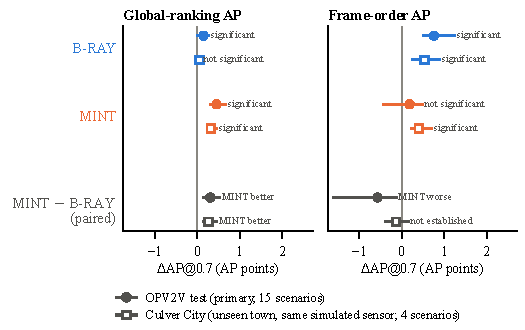
\includegraphics[width=\columnwidth]{figures/forest.pdf}
\caption{Main result. Mean $\Delta$AP@0.7 over the four original attacks, in AP points, under both AP
definitions; filled circles: OPV2V test (primary), open squares: Culver City (secondary). Bars are 95\%
scenario-bootstrap CIs. Labels on B-RAY and \mint: significant or not after Holm correction (one-sided test, so a
bar that touches zero can still be significant). Labels on the paired row: the statement written in advance,
chosen by whether the CI lies above zero, below zero, or includes it.}
\label{fig:forest}
\end{figure}

\subsection{Which attacks does it help against?}
\label{sec:byattack}
Table~\ref{tab:conditions} breaks the results down by condition.

\textbf{Removal attacks.} This is where \mint{} differs most from a box filter. Under global-ranking AP, \mint{}
is the only defense whose CI lies above zero on all four removal conditions, on both sets. B-RAY's effect on
removal is zero or slightly negative, as expected: a filter that can only delete boxes cannot bring back a removed
car. The strongest stealth removal$^\dagger$ makes the difference plain. It costs the undefended receiver
\LossGlobPgdRemStStrong\pts{} on the test, and \mint{} gains \dGlobPgdRemStStrongMINT\pts{}
\ciGlobPgdRemStStrongMINT, a recovery of \RecGlobPgdRemStStrongMINT; on Culver City the attack costs
\CulLossGlobPgdRemStStrong\pts{} and the recovery is \CulRecGlobPgdRemStStrongMINT. At this strength, dropping all
senders (ego-only) gains about as much (\dGlobPgdRemStStrongEgo{} and \CulDGlobPgdRemStStrongEgo\pts), because the
attack destroys more than cooperation adds; \mint{} reaches this level while keeping the benign senders.

\textbf{Spoofing and shifting.} Both ray-based defenses help against added and moved cars. B-RAY's gains are
largest here under frame-order AP (\dFrameSpoofFeatBRAY\pts{} on the test for feature spoofs), where deleting
low-score fake boxes pays off most.

\textbf{Every condition.} Under global-ranking AP, \mint's CI lies above zero in all \NumConditions{} conditions
of the test, clean frames included, and in all but two on Culver City. Under frame-order AP this does not hold:
on the test, \mint{} loses \dFrameCleanMINT\pts{} on clean frames, and its removal gain is resolved only at the
strongest level.

\begin{table*}[!t]
\caption{$\Delta$AP@0.7 against no defense per condition for B-RAY and \mint, OPV2V test (primary) and Culver
City (secondary), both AP definitions, in AP points. \textbf{Bold}: 95\% scenario-bootstrap CI above zero;
\textit{italic}: CI below zero. CIs and the other defenses are in Tables~\ref{tab:full-g} and~\ref{tab:full-f}.
$^\dagger$Added after seeing development results.}
\label{tab:conditions}
\centering
\footnotesize
\setlength{\tabcolsep}{4pt}
\begin{tabular}{lcccccccc}
\toprule
\tabin{tables/tab_conditions.tex}
\bottomrule
\end{tabular}
\end{table*}

\subsection{Which component carries the recovery?}
\label{sec:ablation}
The ablation \mint-noREMOVE keeps every rule except one: a REMOVE effect can never switch a sender off. On the
strongest stealth removal its gain collapses from \dGlobPgdRemStStrongMINT{} to
\dGlobPgdRemStStrongMINTNoRem\pts{} on the test, and from \CulDGlobPgdRemStStrongMINT{} to
\CulDGlobPgdRemStStrongMINTNoRem\pts{} on Culver City. The REMOVE test, which asks whether the receiver's rays
stop where a sender made a car disappear, carries the recovery of removed objects.

The same test is also the main source of \mint's mistakes. On clean test frames, \mint{} switches off
\MintCleanGated{} of \MintCleanUnits{} units, and \MintCleanFalseSwitch{} of them were useful according to the
ground-truth labels (Appendix~\ref{app:extra}); \MintCleanFalseSwitchRemove{} of these come from REMOVE verdicts.
Without REMOVE, only \MintNoRemCleanFalseSwitch{} useful units are switched off, and the mean gain on the four
original attacks is \HeadGlobMINTNoRem{} (global ranking) and \HeadFrameMINTNoRem\pts{} (frame order). The REMOVE
test is thus both \mint's strength and its main cost.

\subsection{What is not defended?}
\label{sec:limits}
\textbf{Receiver-blind spoofs.} No defense recovers more than 0.10 of the loss caused by the receiver-blind spoof,
on either set and under either AP definition. Of the \RealizedSpoofBlind{} spoofs that changed the output on the
test, \BlindRealizedLowRay{} landed where the receiver had fewer than three rays, and \BlindRealizedKnownHit{}
touched a unit the receiver could check (Culver City: \CulBlindRealizedLowRay{} of \CulRealizedSpoofBlind, and
\CulBlindRealizedKnownHit). A ground-truth reference that switches off every harmful unit of the attacker would
recover \OracleRecSpoofBlind{} of the loss, but only \VisOracleRecSpoofBlind{} if it may act only where the
receiver can check (frame-order AP).

\textbf{Feature-statistics checks.} B-NORM catches the plain PGD attacker on \CatchPgdUnt{} of frames, but the
stealth attacker on \CatchPgdUntSt, on both sets. It also flags the benign sender on \CatchClean{} (test) and
\CulCatchClean{} (Culver City) of clean frames with a sender, against \BnormFalseFlagH{} on the development data
where its threshold was set, and so lowers the mean of the four original attacks by \HeadGlobBNORM{} and
\CulHeadGlobBNORM\pts. Against optimized attacks, B-RAY recovers at most \RecFramePgdUntStStrongBRAY{} (test) and
\CulRecFramePgdUntBRAY{} (Culver City) of any PGD attack's loss.

\subsection{What does it cost?}
\label{sec:costs}
\textbf{Accuracy on clean frames} (Table~\ref{tab:clean}, Appendix~\ref{app:tables}). B-RAY's relative clean
loss stays inside the 1\% bound on both sets and under both definitions. \mint's depends on the AP definition:
\CleanGlobMINT{} under global ranking (a small gain) but \CleanFrameMINT{} under frame order on the test, the
price of its false switch-offs; on Culver City it is \CulCleanGlobMINT{} and \CulCleanFrameMINT. B-NORM's false
alarms cost \CleanGlobBNORM{} and \CulCleanGlobBNORM.

\textbf{Computation.} \mint{} decodes once per sender, so its cost grows with the number of vehicles. On our CPU,
the median time it adds to the receiver's own perception is \OvDenseTwoPfifty, \OvDenseThreePfifty{} and
\OvDenseFourPlusPfifty{} with $n=2$, $3$ and ${\ge}4$ agents on the test (Table~\ref{tab:runtime}). B-RAY needs
no extra decode.

%======================================================================
\section{Discussion}
\label{sec:discussion}
%======================================================================
% ~1 page. Interpret; do not restate tables.
\subsection{Why receiver-side verification helps, and where it cannot}
The results support the idea behind \mint: a sender can edit its message, but not the receiver's laser rays.
Whether rays stop on a reported car or pass through it does not depend on how convincing the message looks. This
is why the stealth removal attack, which evades the feature-statistics check completely, is still partly undone
by \mint{} (recovery \RecGlobPgdRemStMINT{} at $r=0.25$ and \RecGlobPgdRemStStrongMINT{} at the strongest level on
the test).

The counterfactual turns this evidence into recovery. A box filter sees only the final output, so it can delete a
fake car but cannot restore a missing one. When a sender makes a car disappear, the car is still present in the
decode without that sender, and the receiver's rays stopping on it show that it is real; switching the sender off
in that tile brings the car back. This is the clearest result of the paper, and the ablation confirms that the
REMOVE test is responsible.

The same reasoning marks the limit. Rays can only judge what the receiver can see, and the receiver-blind spoof
placed almost all of its fakes where they could not. Since even a ground-truth reference restricted to visible
regions does little better, this is a limit of the evidence, not of the decision rule. Closing it needs evidence
from elsewhere, such as other benign vehicles' scans, which brings back the question of whom to trust.

\subsection{Why the ranking depends on the AP definition}
The two AP definitions differ in one respect: where a low-score error is charged. Under global ranking it sits at
the tail of one long list and costs little. Under frame order it is charged at its frame's position and lowers the
precision of every later frame. The same feature spoof therefore costs \LossGlobSpoofFeat\pts{} under global
ranking but \LossFrameSpoofFeat\pts{} under frame order.

The two defenses make different kinds of low-score changes. B-RAY deletes low-score fakes, which helps little
under global ranking but a lot under frame order. \mint's occasional false switch-offs remove a few correct
boxes, which costs almost nothing under global ranking but is charged in full under frame order. Together these
effects flip the comparison. Neither definition is wrong; they weight errors differently. A ranking between
cooperative-perception defenses can therefore depend on an evaluation setting that papers rarely state, and we
recommend reporting which definition is used, and preferably both.

\subsection{Transfer to an unseen town}
Culver City tests whether the findings depend on the town in which the method was developed. The main pattern
carried over: \mint{} again gained significantly, again gained on all four removal attacks, and its comparison with
B-RAY again had the same signs under the two AP definitions. Only B-RAY's small global-ranking gain did not. The
detector itself performs worse there (clean frame-order AP of \CulAPCleanFrame{} against \APCleanFrame), so this is
a real change of conditions. It is not a test of real sensors, however, and with four scenarios its intervals are
wide.

\subsection{Practical implications}
Physical verification and simpler filtering are tools for different attacks. B-RAY is cheap and handles added
cars well; \mint{} is needed when objects are removed. This suggests a hybrid that uses B-RAY for added objects and
only \mint's REMOVE test for removals; we have not tested it. Two costs matter in practice: false switch-offs,
which are local but not free, and computation, which grows with the number of senders. Running the counterfactual
only when a cheap trigger fires reduces the latter but needs further work before it can be trusted for accuracy.

\subsection{Limitations and threats to validity}
\textbf{Attacker.} We assume a single, non-colluding attacker. Two colluding senders could both add the same fake
car; removing one at a time would leave it in place. No attack was optimized against the ray test itself, for
example by placing fakes where fewer than four rays cross them.

\textbf{Detector and data.} We evaluate one detector, AttFuse; the exactness of the tile-by-tile output relies on
its per-pixel fusion, and detectors that mix information across space, such as V2X-ViT~\cite{xu2022v2xvit}, would
need it re-checked. All data are simulated. Real LiDAR misses dark or glass surfaces (more UNKNOWN regions) and
returns from vegetation or spray (false support), and real-world datasets~\cite{xu2023v2v4real,luo2025mixedsignals}
were not evaluated. We assume the receiver's sensor is honest, which physical spoofing~\cite{cao2019advlidar}
would break.

\textbf{Baselines and statistics.} We did not run learned or consensus defenses, and make no claim relative to
them. The bootstrap $p$-value is not calibrated under a null hypothesis, and percentile intervals over 15 or 4
scenarios may be too narrow. Attack levels, the primary and the stealth attacks were set on development data; the
test was run once and cannot be used to tune anything further.

%======================================================================
\section{Conclusion and Future Work}
\label{sec:conclusion}
%======================================================================
% ~0.3 page. No limitations list here.
Cooperative perception helps a vehicle see what its own sensors cannot, but it also lets a sender change what the
receiver detects. This paper asked whether the receiver can check each sender's influence with evidence the
sender cannot forge: its own LiDAR rays. We proposed \mint, which compares the receiver's detections with and
without each sender, region by region, and switches a sender off only where the rays clearly contradict it.

In a pre-registered evaluation on OPV2V, physical verification helped. A simple ray-based box filter already
improved robustness, and \mint{} went further against removal: it was the only defense with a clearly positive
gain on all four removal attacks, on the test and in an unseen town. Whether \mint{} beats the box filter overall
depends on how AP is computed, so the evaluation setting itself can decide a comparison between defenses. For
cooperative perception to be trusted, a received message should not only look plausible; its effect should agree
with what the receiver can physically observe.

Future work should validate this on real-sensor data~\cite{xu2023v2v4real,luo2025mixedsignals}, test attackers
that target the ray test or collude, find evidence for regions the receiver cannot see, and reduce cost, for
example by combining a box filter for added objects with \mint's removal test and running the counterfactual only
when needed.

\section*{Data and Code Availability}
Code, pre-registration files, decision record, result files and analysis scripts are available at
\url{https://github.com/lokrim/Mint}. The OPV2V test ran on the code frozen at commit \texttt{c883753}; the Culver
City evaluation was committed at \texttt{d48fde8}, before its data were downloaded. The SHA-256 checksums of the
result files begin with \texttt{70324a707f23e20b} and \texttt{4b6823ba3603420a} (OPV2V test) and
\texttt{fa6325dee8058bac} and \texttt{5d4481334d983c9c} (Culver City).

\bibliographystyle{IEEEtran}
\bibliography{refs}

%======================================================================
% Supplementary material (after the references; not counted in the 8--9 page target)
%======================================================================
\clearpage
\appendices

\section{Implementation details}
\label{app:impl}
\textbf{PGD.} The attacker perturbs its features at all three scales within
$\|\delta_k\|_\infty\le\epsilon_k=r\,\sigma_k$, where $\sigma_k$ is the standard deviation of clean sender
features on the validation set. Starting from a uniform random $\delta_k$, it takes ten sign-gradient steps of size
$\eta_k=\epsilon_k/4$:
\begin{equation}
\delta_k^{t+1}=\Pi_{\mathcal{B}_k}\!\big(\delta_k^{t}+\eta_k\,\mathrm{sign}\,\nabla_{\delta_k}\mathcal{L}(\delta^{t})\big),
\label{eq:pgd}
\end{equation}
with $\mathcal{B}_k=\{\delta:|\delta|\le\epsilon_k,\ f_{1,k}+\delta\ge 0\}$, so that features stay non-negative.
The loss uses the clean fused output as pseudo-labels, never ground truth. The untargeted attack maximizes the
classification and regression loss on all anchors; the removal attack minimizes the scores of the clean boxes.

\textbf{Stealth projection.} After every step, and after the random start, each scale $k$ is projected onto
the box $[\ell_k,\epsilon_k]$ with $\ell_k=\max(-\epsilon_k,-f_{1,k})$, intersected with B-NORM's bound on the mean
magnitude. With $m_k(\lambda)$ the mean of $f_{1,k}+\mathrm{clip}(\delta_k-\lambda,\ell_k,\epsilon_k)$, the
exact Euclidean projection is
\begin{equation}
\begin{split}
\delta_k&\leftarrow \mathrm{clip}\big(\delta_k-\lambda_k,\ \ell_k,\ \epsilon_k\big),\\
\lambda_k&=\min\big\{\lambda\ge 0:\ m_k(\lambda)\le 0.95\,\tau_k\,\overline{|f_{0,k}|}\big\},
\end{split}
\label{eq:stealth}
\end{equation}
with $\lambda_k$ found by bisection. The factor $0.95$ keeps a small safety margin below B-NORM's threshold.
Frames where no such perturbation exists are not attacked and are scored as clean. On the OPV2V test this
happened on \InfeasiblePgdUntSt, \InfeasiblePgdRemSt, \InfeasiblePgdUntStStrong{} and
\InfeasiblePgdRemStStrong{} of \WithSenderPgdRemSt{} sender frames for the four stealth conditions; on Culver
City on \CulInfeasiblePgdUntSt, \CulInfeasiblePgdRemSt, \CulInfeasiblePgdUntStStrong{} and
\CulInfeasiblePgdRemStStrong{} of \CulWithSender.

\textbf{Ray test.} The core of a box is the box shrunk horizontally by 15\% of each side (at least $0.15$\,m),
trimmed by $0.3$\,m at the bottom and $0.1$\,m at the top. A return is compared with the box enlarged by
$0.2$\,m, with a range tolerance of $0.05$\,m plus 1\% of the range.

\textbf{Runtime.} Table~\ref{tab:runtime} reports the time each defense adds per frame, relative to the
receiver's own perception, as the median (p50) and 95th percentile (p95) over frames, on \TimingMachine{} with
CPU only. ``Full'' is \mint{} as described in Section~\ref{sec:method}. ``Triggered'' is a cheaper variant that
runs the counterfactual only when a fast trigger fires; it is reported for cost only, because it was not exact on
development data and no accuracy number uses it.

\begin{table}[!htb]
\caption{Time added per frame relative to receiver-only perception, p50 / p95 in \%, by number of agents $n$
(\TimingMachine, CPU only). Base: receiver perception p50 in seconds. Culver City has $n\le 3$.}
\label{tab:runtime}
\centering
\footnotesize
\setlength{\tabcolsep}{4pt}
\begin{tabular}{@{}llrcccc@{}}
\toprule
\tabin{tables/tab_runtime_both.tex}
\bottomrule
\end{tabular}
\end{table}
\FloatBarrier

\section{Ground-truth harm labels}
\label{app:extra}
To see what \mint{} switches off, we label every decision unit offline
with ground truth. With Hungarian matching at BEV IoU${}\ge 0.5$ over the boxes centred in tile $u$,
\begin{equation}
\begin{split}
L_u(Y)&=n_{\mathrm{FP}}+n_{\mathrm{FN}}+\tfrac12\textstyle\sum_{\mathrm{TP}}(1-\mathrm{IoU}),\\
D_{i,u}&=L_u(Y^{+})-L_u\big(Y^{-}(i,u)\big),
\end{split}
\label{eq:harm}
\end{equation}
where $n_{\mathrm{FP}}$ and $n_{\mathrm{FN}}$ count the false positives and false negatives in the tile, the
sum runs over its true positives (TP), and $Y^{-}(i,u)$
is the output with sender $i$ switched off in tile $u$. A unit is HARMFUL if $D_{i,u}>0.5$, USEFUL if
$D_{i,u}<-0.5$, and NEUTRAL otherwise. Switching off a USEFUL unit is a \emph{false switch-off}. No defense ever
sees these labels.
\FloatBarrier

\section{Pre-registration history}
\label{app:prereg}
Every rule below was written down and committed before the data it governs were opened. The full record of
these decisions is part of the released repository.

\textbf{Development.} The design set was used to build the method. The validation set was then held out as a
check of the frozen method and was opened afterwards. The first registered plan made our method the primary
hypothesis.

\textbf{How B-RAY became the primary.} Before any B-RAY result on the validation set existed, we fixed a rule
for what would happen next. If the 95\% CI of ``our method minus B-RAY'' on the validation set (frame-order AP)
lay above zero, our method would stay primary. Otherwise, B-RAY would become primary, and the comparison with
our method would become the key secondary question. On the validation set the difference was negative
(\DevHFrameRmB\pts\dev), so B-RAY became the primary. The second version of the plan added the Holm co-test of
both methods against no defense.

\textbf{Two AP definitions.} An audit before the test then found that the sign of this difference on the
validation set depends on the AP definition (Table~\ref{tab:devtest}). Rather than switch the primary a second
time, the final plan requires the success rule to pass under \emph{both} definitions, quotes headline numbers in
global-ranking AP, and reports ``AP-definition-dependent'' where the two disagree. The final plan also added
B-NORM and the PGD attacks. The stealth attacks were designed on the validation set after the plain PGD results
there.

\textbf{Post hoc changes.} Two strong stealth levels ($r=1.0$, $^\dagger$) were added after seeing results on
the validation set; they never enter a criterion. A software bug crashed the first test attempt before any
result was written; it was fixed without changing any method, condition or criterion. An early 10\% latency
budget was dropped as a pass or fail criterion. An early plan to report calibrated probabilities was dropped
when its calibration data became the validation set, which is why the Wilson interval is used only as a
resolvability margin, not as a probability.

\textbf{Culver City.} After the test, the unseen-town evaluation was planned and committed before any of its
data were downloaded, and its results are reported as secondary and descriptive.

\textbf{Development versus test.} \label{app:devtest} Table~\ref{tab:devtest} places the OPV2V test next to the two development sets. These are development
numbers, not test results. The sets were small (design: \DevTScenarios{} scenarios, validation:
\DevHScenarios), the validation set had only $n=\DevHN$ agents, and B-RAY was selected on it. Gains are smaller
on the test than on the validation set under both AP
definitions, but the sign pattern of ``our method minus B-RAY'' is the same.

\begin{table}[!htb]
\caption{Development sets (design and validation) vs.\ OPV2V test: mean $\Delta$AP@0.7 over the four original
attacks in AP points with 95\% scenario CI. G = global-ranking AP, F = frame-order AP. Development numbers are
not test results.}
\label{tab:devtest}
\centering
\scriptsize
\setlength{\tabcolsep}{2.2pt}
\begin{tabular}{@{}lccc@{}}
\toprule
\tabin{tables/tab_dev_vs_test.tex}
\bottomrule
\end{tabular}
\end{table}
\FloatBarrier

\section{Additional results}
\label{app:tables}
\label{app:full}
This appendix collects the tables behind the main text: the data sets (Table~\ref{tab:splits}), the attack
conditions (Table~\ref{tab:attacks}), the full pre-registered verdict shown in Fig.~\ref{fig:forest}
(Table~\ref{tab:verdict}), the clean-frame cost (Table~\ref{tab:clean}), and every defense in every condition
under both AP definitions (Tables~\ref{tab:full-g} and~\ref{tab:full-f}).

\textbf{By number of agents.} Under frame-order AP (CIs from a bootstrap over blocks of 10 frames), B-RAY's mean gain on the OPV2V test falls from
\ByNTwoBRAY\pts{} \ByNTwoBRAYCI{} at $n=2$ to \ByNFourPlusBRAY\pts{} \ByNFourPlusBRAYCI{} at $n\ge 4$, and
\mint's from \ByNTwoMINT{} to \ByNFourPlusMINT\pts{} ($n\ge 4$ covers only \ByNFourPlusScen{} scenarios). On
Culver City, B-RAY gains \CulByNTwoBRAY\pts{} \CulByNTwoBRAYCI{} at $n=2$ (\CulByNTwoScen{} scenarios) and
\CulByNThreeBRAY\pts{} \CulByNThreeBRAYCI{} at $n=3$ (\CulByNThreeScen{} scenario), and \mint{}
\CulByNTwoMINT{} and \CulByNThreeMINT\pts. These strata are descriptive.

\begin{table}[!htb]
\caption{Data sets. The OPV2V test is the primary, one-time evaluation. Culver City, an unseen town with the
same simulated sensor, is a secondary evaluation run once after the test. Design and validation are development sets.
Scen.\ = scenarios; $n$ = number of agents per frame.}
\label{tab:splits}
\centering
\footnotesize
\setlength{\tabcolsep}{4pt}
\begin{tabular}{@{}lrrcp{4.05cm}@{}}
\toprule
\tabin{tables/tab_splits.tex}
\bottomrule
\end{tabular}
\end{table}

\begin{table}[!htb]
\caption{Attack conditions. Real.: frames on which the attack changed the undefended output, out of
\WithSenderSpoofFeat{} OPV2V test frames and \CulWithSender{} Culver City frames with a sender. Loss: drop in
AP@0.7 caused by the attack, in AP points, under global-ranking (G) and frame-order (F) AP. PGD levels are $r$;
st.\ = stealth PGD. $^\dagger$Added after seeing development results.}
\label{tab:attacks}
\centering
\footnotesize
\setlength{\tabcolsep}{2.6pt}
\begin{tabular}{@{}lrrrrrr@{}}
\toprule
\tabin{tables/tab_attacks_both.tex}
\bottomrule
\end{tabular}
\end{table}

\begin{table}[!htb]
\caption{Clean-frame cost. Top: relative AP@0.7 loss on clean frames (positive = loss) with 95\% scenario CI,
under global-ranking (G) and frame-order (F) AP. Bottom, what each defense removes on clean frames: B-RAY, boxes
dropped / boxes (real cars among them); \mint{} and \mint-noREM, units switched off / units (useful ones among
them); B-NORM, benign sender flagged / sender frames.}
\label{tab:clean}
\centering
\scriptsize
\setlength{\tabcolsep}{3.5pt}
\begin{tabular}{@{}lcccc@{}}
\toprule
\tabin{tables/tab_clean_both.tex}
\bottomrule
\end{tabular}
\end{table}

\begin{table*}[!t]
\caption{Pre-registered verdict on the four original attacks: mean $\Delta$AP@0.7 in AP points with 95\%
scenario-bootstrap CI and one-sided bootstrap $p$-value. OPV2V test: confirmatory; Culver City (unseen town, same
simulated sensor, 4 scenarios): the same rule applied descriptively. The two sets are never pooled.
$^\ast$Statement written in advance: the counterfactual method ``improves over'' or ``performs worse than'' the box
filter, or its benefit ``is not established''.}
\label{tab:verdict}
\centering
\footnotesize
\setlength{\tabcolsep}{6pt}
\begin{tabular}{@{}lcccc@{}}
\toprule
\tabin{tables/tab_verdict_both.tex}
\bottomrule
\end{tabular}
\end{table*}

\begin{table*}[!t]
\caption{Every defense in every condition, \textbf{global-ranking AP}: $\Delta$AP@0.7 vs.\ no defense in AP
points, with 95\% scenario-bootstrap CI. Bold: CI above zero; italic: CI below zero. Culver City is the unseen
town (same simulated sensor, 4 scenarios, wide CIs); the two sets are never pooled. PGD levels are $r$; st.\ =
stealth PGD. $^\dagger$Added after seeing development results.}
\label{tab:full-g}
\centering
\scriptsize
\setlength{\tabcolsep}{3pt}
\begin{tabular}{@{}lccccc@{}}
\toprule
\tabin{tables/tab_full_global.tex}
\bottomrule
\end{tabular}
\end{table*}

\begin{table*}[!t]
\caption{As Table~\ref{tab:full-g}, \textbf{frame-order AP} (the OpenCOOD default).}
\label{tab:full-f}
\centering
\scriptsize
\setlength{\tabcolsep}{3pt}
\begin{tabular}{@{}lccccc@{}}
\toprule
\tabin{tables/tab_full_frame.tex}
\bottomrule
\end{tabular}
\end{table*}

\end{document}
